% !TEX root = .

\documentclass[a4paper, 12pt, oneside, BCOR1cm,toc=chapterentrywithdots, hidelinks, parskip]{scrbook}
\usepackage{scrhack}

\usepackage[a4paper]{geometry}
\usepackage{textcomp}
\usepackage{longtable}
\usepackage{booktabs}
\usepackage{tabularx}
\usepackage{rotating}
\usepackage{float}
%\usepackage{tabu}

\usepackage[ngerman, english]{babel}
\usepackage[utf8]{inputenc}
\usepackage{graphicx} 
\usepackage{acronym}
\usepackage{url}           	 
\usepackage{hyperref} 	
\usepackage{listings, color}	% for source code
\usepackage{scrlayer-scrpage}	% header and footer line
\usepackage{acronym}
\usepackage[ruled,vlined,algochapter]{algorithm2e}
%\usepackage[nottoc, notlof, notlot]{tocbibind}
\usepackage{blindtext}
\usepackage{mathtools}
\newcommand*\mean[1]{\bar{#1}}
\usepackage{chngcntr}
\usepackage{adjustbox}
\usepackage{indentfirst}
\setlength{\parindent}{1em}
\setlength{\parskip}{1ex plus 0.2ex}
\usepackage{amssymb}
\makeatletter
\newcommand\notsotiny{\@setfontsize\notsotiny\@vipt\@viipt}
\makeatother


\counterwithout{figure}{chapter}
\counterwithout{table}{chapter}
\counterwithout{algocf}{chapter} 
%\counterwithout{lstlisting}{chapter}
\AtBeginDocument{% the counter is defined later
  \counterwithout{lstlisting}{chapter}%
}
\renewcommand\lstlistingname{Code Fragment}
\lstdefinelanguage{json}{
  basicstyle=\normalfont\ttfamily,
  showstringspaces=false,
  breaklines=true,
  frame=single,
  literate=
   *{"dataSchema"}{{{\color{teal}{"dataSchema"}}}}{10}
   {"AVRO"}{{{\color{cyan}{"AVRO"}}}}{4}
   {"KAFKA\_STRUCT"}{{{\color{purple}{"KAFKA\_STRUCT"}}}}{12}
   {"globalConfig"}{{{\color{magenta}{"globalConfig"}}}}{12}
   {"anonymizers"}{{{\color{yellow}{"anonymizers"}}}}{11}
    {"streamProperties"}{{{\color{orange}{"streamProperties"}}}}{16},
}

%for adding comments
\usepackage{verbatim}

% for tables
\usepackage{multirow}
\newcolumntype{C}[1]{>{\centering\arraybackslash}p{#1}}
\newcolumntype{L}[1]{>{\raggedright\arraybackslash}p{#1}}
\usepackage[table]{xcolor}
\definecolor{lightred}{rgb}{1, 0.8, 0.8} 
\definecolor{lightyellow}{rgb}{1, 1, 0.8}
\definecolor{lightblue}{rgb}{0.8, 0.9, 1}
\definecolor{lightgreen}{rgb}{0.8, 1, 0.8}

\usepackage{xcolor}
\definecolor{purple}{HTML}{6929c4} 
\definecolor{magenta}{HTML}{9f1853} 
\definecolor{green}{HTML}{198038} 
\definecolor{yellow}{HTML}{b28600} 
\definecolor{orange}{HTML}{8a3800} 
\definecolor{teal}{HTML}{009d9a} 
\definecolor{cyan}{HTML}{1192e8} 


% header and footer line - no header & footer line on pages where a new chapter starts
\pagestyle{scrheadings}
% TU Berlin logo at header
%\chead{
\includegraphics[width=1.2cm]{./img/TU-Berlin-Logo.pdf} 
%}

\usepackage{tikz}
\usetikzlibrary{shapes, arrows, positioning, calc}

\begin{document}

\frontmatter
%Titlepage
\thispagestyle{empty}
\begin{center}

\begin{figure}[t]
    \centering
    
\includegraphics[width=3cm]{./img/TU-Berlin-Logo.pdf}%
%    \qquad
%    \includegraphics[width=3.3cm]{dima_logo.png}%
\end{figure}

%\vspace*{0.2cm}
{\LARGE \textbf{Technische Universit\"at Berlin}}

\vspace{0.5cm}

{\large Chair of Database Systems and Information Management\\[1.6mm]}
%{\large Fachgebiet Datenbanksysteme und Informationsmanagement\\[5mm]}

%Fakult\"at IV\\
%Einsteinufer 17\\
%10587 Berlin\\
%https://www.dima.tu-berlin.de\\

\vspace{2.0cm}

{\LARGE Master's Thesis}\\

\vspace{2.45cm}
{\LARGE \textbf{Anonymized Access Control for Distributed Event Stores}}\\
%\vspace*{0.3cm}
%{\LARGE \textbf{second Line}}\\
\vspace{1.0cm}
%{\LARGE Firstname Lastname(s)}
%\vspace*{0.5cm}
Henri Tyl Allgöwer \\
Degree Program: Computer Science\\
Matriculation Number: 454925\\

\vspace*{2.45cm}
\textbf{Reviewers}\\
Prof. Dr. Volker Markl\\
Prof. Dr. Odej Kao\\
\vspace*{0.5cm}
\textbf{Advisor}\\
Rudi Poepsel Lemaitre\\
\vspace{0.5 cm}

\textbf{Submission Date}\\
30.11.2023\\ % 	date of submission
\end{center}


\thispagestyle{empty}
\cleardoublepage
    
%Self-assertion
\newpage

\thispagestyle{empty}

\begin{large}

\vspace*{6cm}

\noindent
Hereby I declare that I wrote this thesis myself with the help of no more than the mentioned literature and auxiliary means.
\vspace{2cm}

\noindent
Berlin, \today

\vspace{3cm}

\hspace*{7cm}%
\dotfill\\
\hspace*{7.5cm}%
\textit{Henri Tyl Allgöwer}

\end{large}
 
\thispagestyle{empty}
\cleardoublepage

% Abstract in Deutsch
\addchap*{Zusammenfassung}
Tipps zum Schreiben dieses Abschnitts finden Sie unter \cite{wallwork_177}

% Abstract
\addchap*{Abstract}
Modern database systems are of incredible importance. Without them, our entire infrastructure would fall apart. Hospitals could no longer properly treat patients, lacking the necessary patient records and treatment history. Banks and financial services would be left unable to execute transactions. Telecommunication services would shut down. These modern database systems often utilize message brokers in combination with stream processing engines. They are capable of accumulating, processing, and distributing data in real-time at an unprecedented rate and volume. With the focus firmly on performance and scalability, data protection has been left behind. A critical oversight as protecting sensitive data is essential in ensuring personal privacy, preventing misuse and fraud, and upholding trust in data handling. At the moment, these database systems provide only very basic access control and lack mechanisms for enforcing privacy policies. Companies often resort to encrypting the data flowing through database systems and focus on external authentification and authorization. Processing encrypted data, however, comes with challenges including computational overhead, added complexity, and performance trade-offs. Decrypting the data again before processing leads back to square one. \par
This thesis introduces a novel model for data anonymization with integrated access control enforcing mechanisms uniquely within modern database systems, more specifically \acfp{DES}. We have realized our model through the development of a new system the \acf{DASH} for Apache Kafka, a leading \ac{DES}. \ac{DASH} is capable of applying a broad variety of anonymization techniques to data streams, uniquely within the database infrastructure. Our tests demonstrate \ac{DASH}'s ability to apply anonymization on individual tuples without introducing performance overhead. We found more complex anonymization techniques, such as those required for achieving k-anonymity on collections of tuples, to be strongly coupled with available system resources. Our evaluation reveals that simpler anonymization techniques are suited for even the highest performance demands, whereas more complex anonymization techniques are more limited in their application.
  
% Acknowledgments  
\addchap*{Acknowledgments}
For recommendations on writing your Acknowledgments see \cite{wallwork_306}.
Thank you to the chair at \ac*{DIMA}

%table of contents
\addtocontents{toc}{\protect\setcounter{tocdepth}{-1}}
\tableofcontents
\addtocontents{toc}{\protect\setcounter{tocdepth}{3}}

%footnote
\newcommand\blfootnote[1]{%
  \begingroup
  \renewcommand\thefootnote{}\footnote{#1}%
  \addtocounter{footnote}{-1}%
  \endgroup
}
%list of figures
\listoffigures

%list of tables
\listoftables



    

    

% List of Abbreviations
\onecolumn
\addchap{List of Abbreviations}
\begin{acronym}[Bash]   
  \acro{ACL}{Access Control List}
  \acro{CCPA}{California Consumer Privacy Act}
  \acro{DASH}{Data Anonymization Stream Handler}
  \acro{DIMA}{Database Systems and Information Management}
  \acro{DAC}{Discretionary Access Control}
  \acro{DES}{Distributed Event Store}
  \acro{GDPR}{General Data Protection Regulation}
  \acro{ICD}{International Statistical Classification of Diseases and Related Health Problems}
  \acro{IoT}{Internet of Things}
  \acro{KNN}{K-Nearest Neighbors}
  \acro{MAC}{Mandatory Access Control}
  \acro{PII}{Personally Identifiable Information}
  \acro{RBAC}{Role Based Access Control}
  \acro{SSE}{Sum of Squared Errors}
\end{acronym}
\onecolumn
\acrodefplural{ACL}{Access Control Lists}

%algorithms
\listofalgorithms
\addcontentsline{toc}{chapter}{List of Algorithms}

%In case, code fragments have to be added
%\renewcommand{\lstlistlistingname}{List of Code Fragments}
%\lstlistoflistings
%\addcontentsline{toc}{chapter}{List of Code Fragments}

\mainmatter % comment single chapters for faster compilation
    
    \chapter{Introduction\label{cha:chapter1}}
Distributed event stores capture, store, and process real-time data streams in distributed environments. They have been widely adopted across various sectors, including Fortune 100 companies, governments, healthcare, and transportation industries \cite{kafka} for their efficient, scalable, and fault-tolerant system design. In the modern data-driven world, the growing demand for comprehensive data privacy policies has resulted in increasingly stringent regulations from governments worldwide \cite{GDPR, CCPA}. However, the underlying infrastructure for distributed event stores to adequately support these policies is markedly lacking \cite{Colombo2015}. This disparity poses a unique challenge, particularly when considering the demands of modern database systems to maintain high performance, characterized by low latency and high throughput.\par
The present work aims to examine what techniques can be effectively employed to ensure privacy and security measures, such as access control and data masking, in distributed event stores. Additionally, it aims to explore what strategies can be developed and implemented to ensure that these privacy and security measures have a minimal impact on the performance of distributed event stores. \par
While there exists a body of work focusing on anonymization and data masking for data streaming \cite{Cao2008, KIDS_zhang, anonymizing_IoT}, there is a noticeable gap in research specifically targeting distributed event stores. 
Furthermore, although there are enterprise technologies for managing data flowing into such systems \cite{privitar}, there is limited literature on techniques designed for data already within distributed event stores. Most notably, the concept of integrating \ac{RBAC} within this framework, where the role assigned determines the level of anonymity accorded to the data, is a completely novel approach. \par
The introduction of access control coupled with anonymization in distributed event stores holds the potential to contribute to more advanced, efficient, and secure data handling. By making such tools accessible and cost-effective, companies might be more inclined to prioritize and invest in user data privacy.\par
The overarching goal of this thesis is to design, implement, and evaluate a management framework for distributed event stores. This framework aims to incorporate \ac{RBAC}, granting administrators the capacity to define levels of data anonymization and specify masking functions. By associating levels of anonymization with the number of additional data streams per original data stream, the framework will facilitate nuanced and customizable data privacy measures. Moreover, this plugin will facilitate the assignment of consumers to streams based on their specific roles, further enhancing granular control over data access and privacy within distributed event stores.\par
The scope of this thesis will primarily encompass the exploration of privacy and security measures in the context of distributed event stores. The thesis will delve into the administrative aspects of these technologies, including the implementation and management of access control and data masking functions. Particular attention will be paid to the role of administrators and the impact of their decisions on the performance of these systems. This includes the computational implications of various anonymization techniques. It will involve an in-depth study of different strategies' performance impacts, aiming to minimize overhead while maintaining robust data privacy. At the same time, this thesis will not specifically address or align with any particular data privacy policy such as the \ac{GDPR} \cite{GDPR}. While the thesis is designed around general principles of data privacy and security, it will not provide policy-specific solutions or address the nuances of any specific regulatory framework. Furthermore, the anonymization of data flowing into or out of distributed event stores is beyond the scope of this thesis. The focus will primarily be on the data within the systems, and not on the methods and protocols for handling data entering or leaving these systems. \par
This thesis introduces the \acf{DASH}, a system architected to process data streams into multiple anonymized versions. This design aims to provide users of distributed event stores with a nuanced granularity of anonymization. A comprehensive survey of anonymization techniques is presented, categorizing these methodologies for practical application in various scenarios. \ac{DASH} includes an extensive library of anonymization techniques, offering users the flexibility to tailor the anonymization process to their specific requirements. Additionally, role-based access control is made available as a separate component to assign anonymized versions to streams. This combination of access control with anonymization variety is not only theoretically robust but also practically applicable. Its synergy is highlighted in our theoretical framework chapter, where we showcase a real-world example. Furthermore, this thesis presents a theoretical model designed to simplify future implementations of anonymized access control across various distributed event stores. \par
In the context of this research, we have tested and evaluated \ac{DASH} in an extensive data pipeline environment. We have found \dots \par
The thesis is structured as follows: in Chapter \ref{cha:chapter2} we conduct a literature review. The theoretical framework is constructed in Chapter \ref{cha:chapter3}. Subsequently, Chapter \ref{cha:chapter4} examines in detail the implementation. Tests and their evaluations are addressed in Chapter \ref{cha:chapter5}. Finally, Chapter \ref{cha:chapter6} presents the conclusion and offers an outlook on future work.

    \chapter{Literature Review\label{cha:chapter2}}

\section{Distributed Event Stores}

\section{Anonymization\label{sec:anon}}

\section{Role Based Access Control}

\section{Privitar}

... should include the following:
\begin{itemize}
    \item definitions / technical terms,
    \item theoretical foundations / principles,
    \item descriptions of algorithms, hardware, software, and/or systems employed.
\end{itemize}



\begin{figure}[h]
\centering
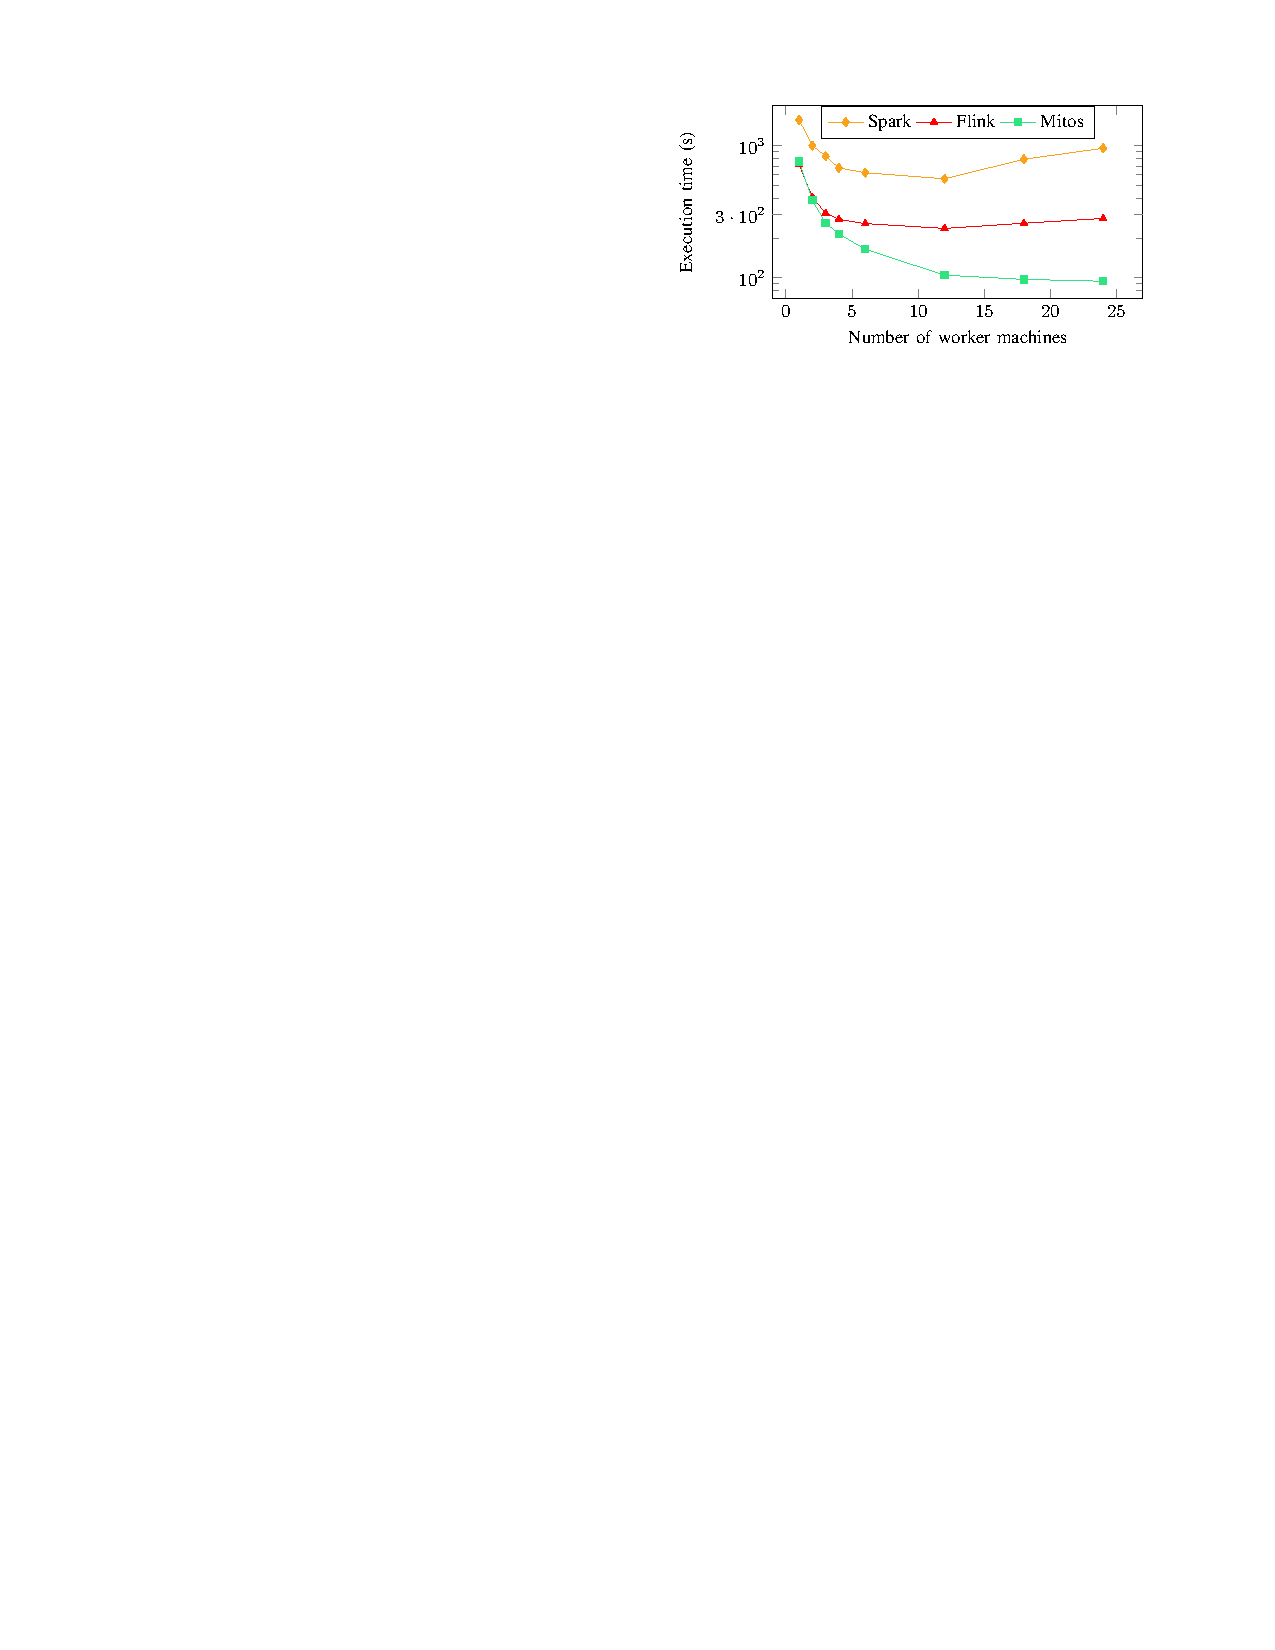
\includegraphics[width=0.6\textwidth]{./img/strong_scaling.pdf}
\caption{Strong scaling for Visit Count\cite{GevayRBMQM21}.}
\end{figure}

% We can leave this out... The advisor can point this out, if it is a concern.
%Suggestion: Figures could be inserted in pdf form to avoid pixelation when the image is magnified.

%This section is intended to give an introduction about relevant terms, technologies and standards in the field of X. You do not have to explain common technologies such as HTML or XML. 



    \chapter{Theoretical Framework\label{cha:chapter3}}

\section{Managing Different Anonymization Granularity}
When planning to integrate anonymization techniques into existing systems, there are many things to consider. First one must understand the data flowing through the system.
Does it include \ac{PII}? Is there further sensitive data? What part of it is necessary for system maintenance? Maybe there is additional data collected for statistics.
Bearing this in mind the next thought would what needs to be anonymized. For this privacy agreements with the user must be taken into account. There may be additional government regulations in place like the \ac{CCPA} in the United States of America or the \ac{GDPR} in the European Union. 
The next course of action is deciding on specific masking functions. As was discussed in \ref{sec:anon} there is a plethora to chose from. It is important to note that all forms of anonymization lead to a loss of information. 
While choosing Blurring or Suppression, two methods that replace attributes with a placeholder, for all critical data fields derived in the previous assessment will ensure that all privacy concerns are addressed, it will also diminish all intelligence gained from collecting this data in the first place. It is questionable if not collecting this type of data in the first place would then be the better solution as it would save storage and computing power. 
An alternative approach would be to invest heavily in the IT security ensuring that no intruder with malicious intent can gain access to sensitive data. Keeping in mind, however, that social engineering attacks are nowadays the most common and effective strategy (SAUCE) giving a guarantee of safety can be impossible. It also stands to reason that the more employees a company has the risk for social
engineering attacks increases. Both of these radical approaches do not seem to adequately solve the problem. Fortunately, there is a way to navigate between these two extremes. An attentive observer of the company's data operations will likely notice that data can and should be restricted similarily to permissions: Only the data needed to furfill the user's duty should be accessible to the user. 
In addition, there are anonymization techniques, which do not lead to total information loss like the two mentioned before. Generalization for example can be employed to significantly reduce the re-identification of individuals, while simultaneously retaining some information.
With data restriction and different anonymization techniques in mind there is a middle ground to be found which maximizes security and minimizes information loss. Consider the following example:

\subsection{Use Case Example}
Hospitals depend on the collection, management and analysis of data to administer the best and most accurate care of their patients. In a modern hospital all data would be stored in a centralized hospital database. 
Here all data for individual patients are brought together. Table \ref{table:dia_patient} shows an exemplary table of patients in the endocrinology ward of a german hospital. Note that the tuple has been shortened to enhance its readability as well as prepended with a header of the corresponding database table.  (A MORE DETAILED VERSION CAN BE FOUND IN THE APPENDIX)


\bigskip 


\begin{table}[ht]
    \begin{center}
    \footnotesize{
        \renewcommand{\arraystretch}{1.5}
        \begin{tabular}{ | c | c | c | c | c | c | c | c | c | c | c | } 
            \hline
            pid & name & zip & sex & age & ins. co. & ins. no. & diag. & gluc. & hba1c & med. \\
            \hline
            1 & F. Ott & 10969 & M & 28 & TK & K15489 & E10 & 22.1 & 8.74 & Insulin \\
            \hline
            2 & L. Lieb & 34127 & F & 59 & AOK & Y41271 & E11 & 16.3 & 7.61 & Metformin \\
            \hline 
            3 & T. Zeit & 70192 & M & 15 & TK & Z17291 & E10 & 23.8 & 8.13 & Insulin \\
            \hline
            4 & H. Lang & 80923 & F & 21 & TK & I79435 & E10 & 18.9 & 7.99 & Insulin \\
            \hline
            5 & J. Putz & 91757 & D & 24 & IKK & Q29751 & E10 & 21.2 & 6.04 & Insulin \\
            \hline
            6 & I. Spies & 60819 & M & 68 & TK & J33921 & E11 & 19.1 & 5.07 & Metformin \\
            \hline
        \end{tabular}
    }
    \caption{Example table of diabetes patients}
    \label{table:dia_patient}
    \end{center}
\end{table}

The header of table \ref{table:dia_patient} shows eleven attributes. First the person id (\textit{pid}), which is the primary key for each patient as it uniquely identifies the patient in the database. Then \textit{name}, zip code (\textit{zip}), \textit{sex} and \textit{age} are included as additional personal information.
This would typically also include the full address not just the zip code, contact information, height as well as weight to adapt the dosage of the medication. The subsequent two attributes include information about the patient's insurance information. 
Insurance companies in Germany are uniquely identified with a nine digit institutional identifier. In the case of the first entry the insurance company (\textit{ins. co.}) has the value 101575519, which matches the identifier of the Techniker Krankenkasse (TK). 
Each client is then assigned a number unique to that insurance company called the insurance number (\textit{ins. no.}). It always starts with a letter followed by digits. Finally, the datum references the medical information. It starts with the diagnosis (\textit{diag.}) classified according to the \ac*{ICD}. 
E10 being the label for Type 1 Diabetes Mellitus, E11 the label for Type 2 Diabetes Mellitus. The most important medical measurement for the treatment of this disease is the current amount of glucose (\textit{gluc.}) in the blood. This determines the quantity of medication (\textit{med.}) to be administered to the patient. For Type 1 Diabetes this is Insulin, for Type 2 it is Metformin. 
Lastly, the table includes an attribute called \textit{hba1c}. This is the body's own three-month average of blood glucose. By means of which diabetes is diagnosed. In this case it is also symbolic for all additional diagnostic findings. 
Glucose and HbA1c are intentionally distinguished as separate attributes in this dataset, despite both being blood-derived metrics, due to their distinct measurement methodologies and relevance in immediate treatment contexts. Glucose can be ascertained with a single drop of blood, providing critical information for the immediate treatment.
Conversely, HbA1c is derived from a complete blood count and does not require instant action. \newline

In a hospital setting, numerous actors engage with the aforementioned dataset. The most straightforward and prominent is the doctor. She will need all data to fulfill her duties. The doctor's letter contains all personal information. The medical data is needed for diagnosis and treatment. 
She will also need to keep the insurance information in mind as the covered treatment options are oftentimes different for each company. Additionally, she will need to write the patient's insurance information on the rescriptions. Only the pid could be omitted, but is debatable if the overhead is worth it, considering the pid can be easily inferred with all the given information.
Therefore, no anonymization to the doctor's data makes the most sense. \\\\
\indent Supporting the doctor is the nurse staff. One of their main tasks is to monitor patients and administer medication. To accomplish this they require the diagnosis, medication and in this case the glucose data. As the HbA1c value is not relevant for the immediate treatment it can be safely ommitted. 
Again insurance information is necessary as nurses typically do have the liberty of administer medication according to their own judgement. This is especially important when considering how understaffed hospitals in Germany are most of the time. On the other hand the patient's personal insurance number does not play into this. As nurses also interact directly with the patients they need some basic personal information like name and sex. 
Pid and zip, however, are not required. Therefore, the data for the nurse staff can be anonymized as shown in Table \ref{table:nurse} without limiting the nurses or losing valuable information. 

\bigskip

\begin{table}[ht]
    \begin{center}
    \footnotesize{
        \renewcommand{\arraystretch}{1.5}
        \begin{tabular}{ | c | c | c | c | c | c | c | c | c | c | c | } 
            \hline
            \cellcolor{lightred} pid & name & \cellcolor{lightred} zip & sex & age & ins. co. & \cellcolor{lightred} ins. no. & diag. & gluc. & \cellcolor{lightred} hba1c & med. \\
            \hline
            \cellcolor{lightred} * & F. Ott & \cellcolor{lightred} * & M & 28 & TK & \cellcolor{lightred} * & E10 & 22.1 & \cellcolor{lightred} * & Insulin \\
            \hline
            \cellcolor{lightred} * & L. Lieb & \cellcolor{lightred} * & F & 59 & AOK & \cellcolor{lightred} * & E11 & 16.3 & \cellcolor{lightred} * & Metformin \\
            \hline 
            \cellcolor{lightred} * & T. Zeit & \cellcolor{lightred} * & M & 15 & TK & \cellcolor{lightred} * & E10 & 23.8 & \cellcolor{lightred} * & Insulin \\
            \hline
            \cellcolor{lightred} * & H. Lang & \cellcolor{lightred} * & F & 21 & TK & \cellcolor{lightred} * & E10 & 18.9 & \cellcolor{lightred} * & Insulin \\
            \hline
            \cellcolor{lightred} * & J. Putz & \cellcolor{lightred} * & D & 24 & IKK & \cellcolor{lightred} * & E10 & 21.2 & \cellcolor{lightred} * & Insulin \\
            \hline
            \cellcolor{lightred} * & I. Spies & \cellcolor{lightred} * & M & 68 & TK & \cellcolor{lightred} * & E11 & 19.1 & \cellcolor{lightred} * & Metformin \\
            \hline
        \end{tabular}
    }
    \caption{Data available for the nurse staff. Note that pid, zip, insurance number and additional medical information have been suppressed as indicated by their cell's light red background.}
    \label{table:nurse}
    \end{center}
\end{table}

In tandem with the stay and medical treatment of the patient, the administartion of the hospital will want to collect the money from the patient's insurance. The insurance company together with the patient's personal insurance number will suffice as identification. 
Administered medication will be imperative as this dictates the amount of money the hospital will get in addition to the fees for the stay. For this the diagnosis will typically have to be added as a suitable reason. No further information is required. Limiting the amount of data here 
is crucial as here the data is exported to a third party. Which means that additional regulations will take effect. Minimizing the data leaving the hospital minimizes security risks. With these strict rules in place the data can be adjusted as seen in Table \ref{table:administration}. \newline 
Note at this point that an unauthorized entity, who has gained access to both the data of the nurse staff and that of the administration, would struggle to correlate the entries. The shared available data fields insurance company, diagnosis and medication are likely generic enough to not point to a singular but to many patients. 

\bigskip

\begin{table}[ht]
    \begin{center}
    \footnotesize{
        \renewcommand{\arraystretch}{1.5}
        \begin{tabular}{ | c | c | c | c | c | c | c | c | c | c | c | } 
            \hline
            \cellcolor{lightred} pid & \cellcolor{lightred} name & \cellcolor{lightred} zip & \cellcolor{lightred} sex & \cellcolor{lightred} age & ins. co. & ins. no. & diag. & \cellcolor{lightred} gluc. & \cellcolor{lightred} hba1c & med. \\
            \hline
            \cellcolor{lightred} * & \cellcolor{lightred} * & \cellcolor{lightred} * & \cellcolor{lightred} * & \cellcolor{lightred} * & TK & K15489 & E10 & \cellcolor{lightred} * & \cellcolor{lightred} * & Insulin \\
            \hline
            \cellcolor{lightred} * & \cellcolor{lightred} * & \cellcolor{lightred} * & \cellcolor{lightred} * & \cellcolor{lightred} * & AOK & Y41271 & E11 & \cellcolor{lightred} * & \cellcolor{lightred} * & Metformin \\
            \hline 
            \cellcolor{lightred} * & \cellcolor{lightred} * & \cellcolor{lightred} * & \cellcolor{lightred} * & \cellcolor{lightred} * & TK & Z17291 & E10 & \cellcolor{lightred} * & \cellcolor{lightred} * & Insulin \\
            \hline
            \cellcolor{lightred} * & \cellcolor{lightred} * & \cellcolor{lightred} * & \cellcolor{lightred} * & \cellcolor{lightred} * & TK & I79435 & E10 & \cellcolor{lightred} * & \cellcolor{lightred} * & Insulin \\
            \hline
            \cellcolor{lightred} * & \cellcolor{lightred} * & \cellcolor{lightred} * & \cellcolor{lightred} * & \cellcolor{lightred} * & IKK & Q29751 & E10 & \cellcolor{lightred} * & \cellcolor{lightred} * & Insulin \\
            \hline
            \cellcolor{lightred} * & \cellcolor{lightred} * & \cellcolor{lightred} * & \cellcolor{lightred} * & \cellcolor{lightred} * & TK & J33921 & E11 & \cellcolor{lightred} * & \cellcolor{lightred} * & Metformin \\
            \hline
        \end{tabular}
    }
    \caption{Data available for the administration. Note that only the insurance information, medication and diagnosis are not suppressed.}
    \label{table:administration}
    \end{center}
\end{table}

Diabetes, which afflicts over ten percent of the global population and demonstrates a rising prevalence, stands as one of the most common chronic diseases worldwide \cite{idf2023,WHODiabetes2023}. Given its mostly non-lethal progression and lifetime dependency on medication, 
it has given rise to a substatial market. As cause, optimal treatment and cure remain subject to research, data of especially newer diabetes patients is in hot demand. To provide this data to research institutes in accordance with the regulations in place the hospital must ensure that no concrete patient can be reidentified. 
Here, advanced anonymization techniques such as K-Anonymization come into place. Each attribute of the data entry can be assigned to one of three categories: personally identifiable, quasi identifying and sensitive attributes. To achieve k anonymity each entry must suppress the personally identifiable attributes, while keeping the sensitive attributes untouched. 
Most importantly the quasi identifiable attributes of each data entry must be the same for at least k - 1 other entries of a data set. This is typically achieving with generalization of these attributes until k entries are found. In this use case the personally identifiable attributes are \textit{pid}, \textit{name} and \textit{insurance number}. 
The quasi indentifying attributes are \textit{zip}, \textit{sex}, \textit{age} and \textit{insurance company}. The medical data comprive the sensitive attributes. A K anonymous version of this data extry is depicted in Table \ref{table:k_anon}. 

\bigskip

\begin{table}[ht]
    \begin{center}
        \footnotesize{
            \renewcommand{\arraystretch}{1.5}
            \begin{adjustbox}{center}
                \begin{tabular}{ | c | c | c | c | c | c | c | c | c | c | c | } 
                    \hline
                    \cellcolor{lightred} pid & \cellcolor{lightred} name & \cellcolor{lightyellow} zip & \cellcolor{lightyellow} sex & \cellcolor{lightyellow} age & \cellcolor{lightyellow} ins. co. & \cellcolor{lightred} ins. no. & diag. & gluc. & hba1c & med. \\
                    \hline
                    \cellcolor{lightred} * & \cellcolor{lightred} * & \cellcolor{lightyellow} XXXXX & M & \cellcolor{lightyellow} {[10 - 70]} & TK & \cellcolor{lightred} * & E10 & 22.1 & 8.74 & Insulin \\
                    \hline
                    \cellcolor{lightred} * & \cellcolor{lightred} * & \cellcolor{lightyellow} XXXXX & M & \cellcolor{lightyellow} {[10 - 70]} & TK & \cellcolor{lightred} * & E10 & 23.8 & 8.13 & Insulin \\
                    \hline 
                    \cellcolor{lightred} * & \cellcolor{lightred} * & \cellcolor{lightyellow} XXXXX & M & \cellcolor{lightyellow} {[10 - 70]} & TK & \cellcolor{lightred} * & E11 & 19.1 & 5.07 & Metformin \\
                    \hline
                    \cellcolor{lightred} * & \cellcolor{lightred} * & \cellcolor{lightyellow} XXXXX & \cellcolor{lightyellow} \{M, F, D\} & \cellcolor{lightyellow} {[10 - 70]} & \cellcolor{lightyellow} ins. co & \cellcolor{lightred} * & E11 & 16.3 & 7.61 & Metformin \\
                    \hline
                    \cellcolor{lightred} * & \cellcolor{lightred} * & \cellcolor{lightyellow} XXXXX & \cellcolor{lightyellow} \{M, F, D\} & \cellcolor{lightyellow} {[10 - 70]} & \cellcolor{lightyellow} ins. co & \cellcolor{lightred} * & E10 & 18.9 & 7.99 & Insulin \\
                    \hline
                    \cellcolor{lightred} * & \cellcolor{lightred} * & \cellcolor{lightyellow} XXXXX & \cellcolor{lightyellow} \{M, F, D\} & \cellcolor{lightyellow} {[10 - 70]} & \cellcolor{lightyellow} ins. co & \cellcolor{lightred} * & E10 & 21.2 & 6.04 & Insulin \\
                    \hline
                \end{tabular}
            \end{adjustbox}
        }
    \caption{K-anonymized data available for external research. The sensitive medical attribtues remains unchanged as indicated by the white cell background. Unlike the personally identifying attributes, which have been suppressed as denoted by the red cell background. The yellow cell background highlights the generalized quasi identifiable attributes. Note that the entries of the first group have unchanged values for the attributes \textit{sex} and \textit{ins. co.}. As all three original entries shared the same value it did not need to be generalized.}
    \label{table:k_anon}
    \end{center}
\end{table}

While the aforementioned diabetes patient use case scenario may appear unique and specific, the aspects and nuances are applicable in numerous contexts. The distinct data requirements for doctors, nurses, administration and research are anticipated to persist, albeit adapted, throughout the entire healthcare industry. 
It is also viable in different sectors. Imagine security levels in government matters, trade secrets and specific customer knowledge in corporations or secrecy of correspondense for the transportation industry. Distributed event stores are utilized across all of these sectors with major players relying on Apache Kafka for their day to day needs \cite{KafkaPoweredBY}. 

\section{Anonymization Techniques}
Data anonymization is a multifaceted process tailored to meet application requirements, user groups and their specific needs. This section first goes in depth into masking functions, the cornerstone of data anonymization. It then explores table based techniques that look at the whole dataset to ensure privacy. In this context a \textit{datum} refers to a single piece of information e.g. a singular entry of a database or any one event of a data stream. Synonymous with it also used the word \textit{tuple}. A tuple is comprived of one or multiple \textit{attributes} (also called \textit{fields}). It is customary for individual tuples to be part of a bigger collection. In the static context they are collected in databases and grouped in tables. Data streams work analogous for dynamic operations. All tuples of the same database table or data stream are required to follow the same pattern. This refers to the sequence of attributes of each tuple. This pattern is fixed in a data schema associated with the table or stream. Sometimes it is appended to each datum in form of a header as seen exemplary in Table \ref{table:dia_patient}. As this substantially increases the size of each datum it is more common to define it once in the initialization step of the database table or data stream. \\
While all forms of anonymization aim to alter the underlying sensitive information, e.g. the tuple's attributes containing perhaps personally identifiying information, in a way that makes it harder if not impossible to reconstruct, they can be further categorized based on their scope of operation:

\begin{itemize}
    \item \textbf{Value-Based} Handles one tuple at a time and replaces the values of attributes independently. 
    \item \textbf{Tuple-Based} Operates on individual attributes of a single tuple, but considers the values of the entire tuple for the change. 
    \item \textbf{Attribute-Based} Extends the view from one tuple to a larger collection or table of data. Evaluates the values of singular attributes of the entire set and collectively makes changes to that attribute accordingly. 
    \item \textbf{Table-Based} Covers a table of data and perceives all attributes of each tuple. Adaptions to multiple attributes simultaneously are common. It can be argued that methods falling under this category are not masking functions but algorithms utilizing many masking functions to achieve anonymization on a table level.  
\end{itemize}

To better illuminate the relationship and hierarchy of the aforementioned categories as well as provide some examples, refer to Figure \ref{fig:hierarchy_mf}. 

\begin{figure}[ht]
    \begin{tikzpicture}[node distance=1.5cm, auto, trim left=-2.5cm]
        % Define block styles
        \tikzstyle{box} = [rectangle, draw, rounded corners, fill=blue!20, text width=5em, text centered, minimum height=3em]
        \tikzstyle{line} = [draw, -latex']

        % Nodes
        
        \node [box, text width=5em, xshift=-1cm] (value) {Value Based};
        \node [box, right=of value, text width=5em] (tuple) {Tuple Based};
        \node [box, right=of tuple, text width=6em] (attribute) {Attribute Based};
        \node [box, right=of attribute, text width=5em] (table) {Table Based};
        \node [box, fill=purple!30, above=of tuple, text width=9em] at ($(value)!0.5!(tuple)$) (semantics1) {Tuple-at-the-time\\ Semantics};
        \node [box, fill=purple!30, above=of attribute, text width=6em] at ($(attribute)$) (semantics2) {Table Semantics};
        \node [box, fill=purple!50, above=of semantics1, text width=6em] at ($(semantics1)!0.5!(semantics2)$) (masking) {Masking Functions};
        \node [box, fill=white, text width=6em, opacity=0, above=of table] at ($(table)$) (reference){};
        \node [box, fill=green!30, above=of reference, text width=7.5em] at ($(reference)$) (anonymizations) {Table Anonymizations};


        % Lists
        \node[below=0.2cm of value] (value_mf) {
            \begin{tabular}{l}
                - Suppression \\
                - Blurring \\
                - Substitution \\
                - Tokenization \\
                - Generalization \\
                - Bucketizing \\
                - Noise Methods
            \end{tabular}
        };

        \node[below=0.2cm of tuple] (tuple_mf) {
            \begin{tabular}{l}
                - Conditional \\ Substitution
            \end{tabular}
        };

        \node[below=0.2cm of attribute] (attribute_mf) {
            \begin{tabular}{l}
                - Aggregation \\
                - Univariate \\ Microaggregation \\
                - Shuffling 
            \end{tabular}
        };

        \node[below=0.2cm of table] (table_mf) {
            \begin{tabular}{l}
                - k-anonymization \\
                - l-diversity \\
                - t-closeness \\
                - Multivariate \\ Microaggregation 
            \end{tabular}
        };

        % Paths
        \path [line] (masking) -- (semantics1);
        \path [line] (masking) -- (semantics2);
        \path [line] (semantics1) -- (value);
        \path [line] (semantics1) -- (tuple);
        \path [line] (semantics2) -- (attribute);
        \path [line] (anonymizations) -- (table);

    \end{tikzpicture}
    \caption{Hierarchy of masking functions}\label{fig:hierarchy_mf} 
\end{figure}

\subsection{Value Based Masking Functions}
Having outlined the structure and dimensions of the various masking functions, it is now time to take a closer look at the functionality and use cases of the examples given in Figure \ref{fig:hierarchy_mf} starting with the value based. \\
\textbf{Suppression} aims to effectively delete the value by replacing the value of an attribute with a meaningless character, most commonly the asterisk \textit{*}. It is important to note, that actually removing the attribute from the tuple or replacing it will a null value would violate the data schema and thus negatively impact operability. The asterisk does the trick while maintaining the data schema. To work Suppression only requires a non-empty set of keys for the attributes that are supposed to be suppressed as parameter. Naturally, it leads to total information loss of the specfified fields. This can be particular useful for fields containing \ac{PII} like a person's home address as exemplary shown in Figure \ref{fig:suppression}. 

\bigskip

\begin{figure}[ht]
    \begin{center}
    \footnotesize{
        \renewcommand{\arraystretch}{1.5}
        \begin{tabular}{|c|}
            \hline
            address \\
            \hline
            Smith Street 3 \\
            \hline
            \end{tabular}
            \quad $\longrightarrow$ \quad
            \begin{tabular}{|c|}
            \hline
            address \\
            \hline
            * \\
            \hline
        \end{tabular}
    }
    \end{center}
    \caption{Example of suppression of an attribute.\label{fig:suppression}}
\end{figure}

A similar approach is applied in \textbf{Blurring}. Here the value of an attribute is replaced with arbitrary characters, typically \textit{X}s. It is distinguishable from Suppression in that not all characters of the value have to be replaced and even the amount of characters can remain the same. Imagine a user at the checkout of an online store that they have already purchased goods at prior to this session. Here the credit card information of that user was saved as part of the agreement from the previous session. The user is then given the option to use that credit card again, with it being specified as a sequence of blurred characters with only the last three digits in plain text as shown in Figure \ref{fig:blurring}. This allows the user to double-check the card information without exposing the credit card number to the network, screen capturers or bystanders. This operation also leads to high information loss but retains some usability of the value. The parameters for Blurring include the keys to blurr as well as optionally the number of characters and whether the amount of characters is to be maintained. Note, that setting the parameters to blur all characters and reduce the amount to one is equal in funtionality to Suppression. 

\bigskip

\begin{figure}[ht]
    \begin{center}
    \footnotesize{
        \renewcommand{\arraystretch}{1.5}
        \begin{tabular}{|c|}
            \hline
            credit card \\
            \hline
            1234 5678 9123 4567 \\
            \hline
            \end{tabular}
            \quad $\longrightarrow$ \quad
            \begin{tabular}{|c|}
            \hline
            credit card \\
            \hline
            XXXX XXXX XXXX X567 \\
            \hline
        \end{tabular}
    }
    \end{center}
    \caption{Example of blurring of an attribute.\label{fig:blurring}}
\end{figure}

\textbf{Substitution} replaces the value of the specified attribute with a predefined substitute. Figure \ref{fig:substitution} shows an example where a name is switched out with an arbitrary fake name from a library. While this masking function leads to substantial information loss, it seemingly maintains the integrity of the data from an outsider's perspective. This can make the data easier to work with, while still ensuring anonymity. As parameters the keys for the attributes that are supposed to be substituted are required in tandem with the intended substitutes. 

\bigskip

\begin{figure}[ht]
    \begin{center}
    \footnotesize{
        \renewcommand{\arraystretch}{1.5}
        \begin{tabular}{|c|}
            \hline
            name \\
            \hline
            Martin Smith \\
            \hline
            \end{tabular}
            \quad $\longrightarrow$ \quad
            \begin{tabular}{|c|}
            \hline
            name \\
            \hline
            John Doe \\
            \hline
        \end{tabular}
    }
    \end{center}
    \caption{Example of substitution of an attribute.\label{fig:substitution}}
\end{figure}

An alternative approach is \textbf{Tokenization}. Here values are also substituted, but not with some arbitrary replacement. Instead, the substitute is a specific token. These tokens can be reversed to restore the original value as long as a secret is known with which the token was created. There are different approaches to achieve this. The first one coming to mind is a database mapping token to the hash of the original value. Only access to the database as well as the hashing function will yield the correct original value from the token. Another approach is to omit the database and instead use a more sophisticated cryptographic algorithm to create the token, essentially encrypting the data. While this masking function manages to preserve the information, it requires substantial overhead in form of storage for the database and/or computing power for the cryptographic algorithms. This costly masking function is usually reserved for highly sensitive data. For instance passwords as illustrated in Figure \ref{fig:tokenization}.

\bigskip

\begin{figure}[ht]
    \begin{center}
    \footnotesize{
        \renewcommand{\arraystretch}{1.5}
        \begin{tabular}{|c|}
            \hline
            password \\
            \hline
            MyPassword1 \\
            \hline
            \end{tabular}
            \quad $\longrightarrow$ \quad
            \begin{tabular}{|c|}
            \hline
            password \\
            \hline
            d9f4c3b72c7935e5 \\
            \hline
        \end{tabular}
    }
    \end{center}
    \caption{Example of tokenization of an attribute.\label{fig:tokenization}}
\end{figure}

One of the most common masking functions is \textbf{Generalization}. Here, the value of an attribute is abstracted to a more general value. This effectively reduces the information, but does not remove it entirely. For example a datum with a residency field could generalize the exact location to a broader one. Instead of Berlin it would read Germany as shown in Figure \ref{fig:generalization}. This could then be even further generalized to Europe and so forth. Typically, entire generalization hierarchies are provided as parameter to facilitate this. It is crucial that these hierarchies are exhaustive of all possible arising values if no default is provided as generalization is ambiguous. These complete generalization hierarchies are required as parameters in addition to their respective attribute key. 

\bigskip

\begin{figure}[ht]
    \begin{center}
    \footnotesize{
        \renewcommand{\arraystretch}{1.5}
        \begin{tabular}{|c|}
            \hline
            residency \\
            \hline
            Berlin \\
            \hline
            \end{tabular}
            \quad $\longrightarrow$ \quad
            \begin{tabular}{|c|}
            \hline
            residency \\
            \hline
            Germany \\
            \hline
        \end{tabular}
    }
    \end{center}
    \caption{Example of the generalization of an attribute.\label{fig:generalization}}
\end{figure}

A special case of Generalization is \textbf{Bucketizing}. It functions similarly, but exclusively for numerical values. Ranges replace specific values in the tuple. Figure \ref{fig:bucketizing} shows an example where the age 27 is bucketized to the range {[20 - 30]}. Only a moderate amount of information is lost with this masking function. To deploy it requires the bucket sizes as well as the keys to the numerical attribute. 

\bigskip

\begin{figure}[ht]
    \begin{center}
    \footnotesize{
        \renewcommand{\arraystretch}{1.5}
        \begin{tabular}{|c|}
            \hline
            age \\
            \hline
            27 \\
            \hline
            \end{tabular}
            \quad $\longrightarrow$ \quad
            \begin{tabular}{|c|}
            \hline
            age \\
            \hline
            {[20 - 30]} \\
            \hline
        \end{tabular}
    }
    \end{center}
    \caption{Example of bucketizing of an attribute.\label{fig:bucketizing}}
\end{figure}

Finally, there are the \textbf{Noise Methods}. Again, these only apply to numerical data. The idea is to modify the original values by adding noise. Typically, this noise is chosen randomly from a distribution. Utilizing the normal distribution with mean 0 it would ensure that the data over a period of time would retain its average and distribution. The standard deviation will then define how much each individual data point can diverge from the original value. The result will invalidate individual tuples but preserve the overall spread of the data in the long run. As an example Figure \ref{fig:noise} shows noise added to two attributes of a tuple. Note that with no loss to the generality one is decreased, while the other increased. 

\bigskip

\begin{figure}[ht]
    \begin{center}
    \footnotesize{
        \renewcommand{\arraystretch}{1.5}
        \begin{tabular}{|c|c|}
            \hline
            height & weight \\
            \hline
            185 & 83 \\
            \hline
            \end{tabular}
            \quad $\longrightarrow$ \quad
            \begin{tabular}{|c|c|}
            \hline
            height & weight  \\
            \hline
            181 & 84\\
            \hline
        \end{tabular}
    }
    \end{center}
    \caption{Example of adding noise.\label{fig:noise}}
\end{figure}

\subsection{Tuple Based Masking Functions}
Extending the scope of operation from independent attributes to the tuple as a whole yields the tuple based masking functions. The most notable candidate is \textbf{Conditional Substitution}. As can be expected the change to the tuple is identical to that of the value based Substitution. The value of the attribute specified by the parameter is changed according to the given substitution dictionary. The key difference, however, is that a change only occurs if a certain condition is met. These are additionally provided as a parameter. They can be specified in a variety of different possible formats like a direct match, a numerical range or even a regular expression. Before showcasing some examples consider the following definitions: \newline
\\
Let $T$ be a tuple defined as a fixed sequence of attributes $a_0$ to $a_n$, $T = (a_0, a_1, \dots, a_n)$. Also, let $i$, $j$ $\in \{0,1, \dots, n\}$. \\

Further, a masking function for conditional substitution $mf_{cs}$ can be defined based on a condition $c$ evaluated on the attribute $a_i$, with a substitute $s$ for the attribute $a_j$:
\vspace{-0.8em}
\[
\begin{aligned}
mf_{cs}(i, c, j, s) &= 
\begin{cases}
    (a_0, \dots, a_{j-1}, s, a_{j+1}, \dots, a_n) & \text{if } c \text{ matches on } a_i \\
    T & \text{else}
\end{cases}
\end{aligned}
\]

Note, a match on c can take on different forms. An example of a conditional substitution masking function for a direct match on the value of one of the attributes is shown in Figure \ref{fig:condiSubValue}. It shows an excerpt of a database table with three entries. Remember that all tuples of a single database table share the same data scheme. For better understanding the header with the attribute's labels is shown in the first row of each table in the figure. It shows that the data in this table has two attributes, \textit{rank} and \textit{salary}. The masking function $mf_{cs}(0, 'Manager', 1, '*')$ is applied to every tuple in the table. It can be read as: if the attribute with index 0 matches on 'Manager', substitute the attribute with index 1 with '*'. Following this logic only one entry in the output was changed, as there was just one match.

\bigskip

\begin{figure}[ht]
    \begin{center}
    \footnotesize{
        \renewcommand{\arraystretch}{1.5}
        \begin{tabular}{|c|c|}
            \hline
            rank & salary\\
            \hline
            Worker & 62 000 \\
            \hline
            Assistant & 45 000 \\
            \hline
            Manager & 135 000 \\
            \hline
        \end{tabular}
        \quad $\xrightarrow{mf_{cs}(0, 'Manager', 1, '*')}$ \quad
        \begin{tabular}{|c|c|}
            \hline
            rank & salary\\
            \hline
            Worker & 62 000 \\
            \hline
            Assistant & 45 000 \\
            \hline
            Manager & * \\
            \hline
        \end{tabular}
    }
    \end{center}
    \caption{Conditional substitution with a direct match condition taking the entire tuple into consideration.\label{fig:condiSubValue}}
\end{figure}

Another example is shown in Figure \ref{fig:condiSubRange}. The condition in this case is a range. Naturally, it can only be applied to numerical attributes since there is a clear ordering of values. In the example the database table shows two attributes: \textit{name} and \textit{age}. The masking function employed is $mf_{cs}(1,[0, 18], 1, 'minor')$. Subsequently, the output shows two changes in the table as two entries match the condition. Note that this time the condition is evaluated on the same attribute as the substitution e.g. $i = j$. 


\bigskip

\begin{figure}[ht]
    \begin{center}
    \footnotesize{
        \renewcommand{\arraystretch}{1.5}
        \begin{tabular}{|c|c|}
            \hline
            name & age \\
            \hline
            John & 45 \\
            \hline
            Frederik & 7 \\
            \hline
            Samatha & 15 \\
            \hline
        \end{tabular}
        \quad $\xrightarrow{mf_{cs}(1,[0, 18], 1, 'minor')}$ \quad
        \begin{tabular}{|c|c|}
            \hline
            name & age \\
            \hline
            John & 45 \\
            \hline
            Frederik & minor  \\
            \hline
            Samatha & minor \\
            \hline
        \end{tabular}
    }
    \end{center}
    \caption{Substitution with a range condition on the basis of only a singular attribute in the tuple. \label{fig:condiSubRange}}
\end{figure}

Finally, Figure \ref{fig:condiSubRegex} shows $mf_{cs}(0,'@example\backslash.com', 1, 0)$ being used as masking function. The attribute \textit{Points} for all entries with the domain 'example.com' in the \textit{Email} attribute, determined through the regular expression \textit{$'@example\backslash.com'$} is set to 0. 

\bigskip

\begin{figure}[ht]
    \begin{center}
    \footnotesize{
        \renewcommand{\arraystretch}{1.5}
        \begin{tabular}{|c|c|}
            \hline
            Email & Points \\
            \hline
            user1@example.com & 150 \\
            \hline
            service@mail.org & 325 \\
            \hline
            john@example.com & 25 \\
            \hline
        \end{tabular}
        \quad $\xrightarrow{mf_{cs}(0,'@example\backslash.com', 1, 0)}$ \quad
        \begin{tabular}{|c|c|}
            \hline
            Email & Points \\
            \hline
            user1@example.com & 0 \\
            \hline
            service@mail.org & 325 \\
            \hline
            john@example.com & 0 \\
            \hline
        \end{tabular}
    }
    \end{center}
    \caption{Regular expression as a condition for the substition as part of a tuple based masking function. \label{fig:condiSubRegex}}
\end{figure}

\subsection{Attribute Based Masking Functions}
Following the hierarchy of masking functions depicted in Figure \ref{fig:hierarchy_mf} this concludes the masking functions with Tuple-at-the-time semantics. Next, the focus shifts towards operations on tables, more specifically on collections of tuples. Before, the masking functions were applied to each tuple individually. The focus is to add more context to the anonymization and in return diminishing the information loss caused by anonymizing altogether. Also, it allows the better handling of outliers. Returning to the generalization example from Figure \ref{fig:generalization}, where the residency 'Berlin' was generalized to 'Germany'. If in an entire table there is only one german resident, it would be easy for an unauthorized party, who has gained access to this table, to reidentify the individual from the output. All the masking operation would have done is cost resources and lead to information loss within the system. This is of course not desirable. Fortunately, edge cases like these are unlikely for data with low spread or high density. And even in data sets with high spread and likelihood of outliers, situations like the aforementioned can be easily avoided with knowledge of the data and the correct choice of masking function for the appropriate edge cases e.g. Suppression. An approach that more complex anonymization techniques like the ones discussed in Section \ref{lit:data_streaming} employ inherently. The subsequent subsection will go into more depth on this as well. For the moment, it is crucial to understand that more input can lead to less information loss and more anonymization reliability. It does, however, come at higher computing cost as the findings in Chapter \ref{cha:chapter5} show. More input in the context of attribute based masking functions refers to more values from multiple tuples for the same attribute. Whithin the scope of this thesis it is essential to highlight the particular interest in data streams being the foundation of distributed event stores as opposed to static databases or bounded datasets. Data streams inherently pose additional challenges due to their unbounded nature. In Section \ref{lit:data_streaming} this has been addressed already and windowing was introduced as a means of discretizing data streams. In this context 'collections of tuples', 'table' and 'window' all refer to this same discretization: a finite number of tuples as working base obtained through windowing operations. It is worth mentioning that the parameters for windowing like window size can be included in the optimization of the anonymization itself. This particular nuance is looked into in Section \ref{sec:parameterOptimization} \newline
Building on this understanding, \textbf{Aggregation} as an attribute based masking function leverages this principle. In essence, aggregation combines multiple values into one single value. This in turn will represent the attribute for all input tuples. This effectively reduces the information of an individual entry but preserves the underlying trend. By merging data it significantly reduces the reidentification probability of a single individual through this attribute. There is a variety of aggregation techniques, but they all have one thing in common. They work only on numerical values. Figure \ref{fig:aggregation} shows an example. The table contains six tuples, each tuple only has one attribute, \textit{age}. The right side of the arrow illustrates the result. Note that the amount of tuples remains unchanged, but now all tuples have the same value for the attribute. Depending on the aggregation type, which is written underneath each column, the values have been combined. The first column shows the sum, the second the median, the third the average, the fourth the maximum value found, the fifth the minimum value found, the sixth the number of input tuples and the last the most frequent value in the input table. 

\bigskip

\begin{figure}[ht]
    \begin{center}
    \footnotesize{
        \renewcommand{\arraystretch}{1.5}
        \begin{tabular}{|*{1}{C{1.2cm}|}}
            
            \hline
            age \\
            \hline
            23 \\
            \hline
            45  \\
            \hline
            26 \\
            \hline
            32  \\
            \hline
            26 \\
            \hline
            27 \\
            \hline
            \multicolumn{1}{c}{} \\
        \end{tabular}
        \quad $\longrightarrow$ \quad
        \begin{tabular}{|*{7}{C{1.2cm}|}}
            \hline
            \multicolumn{7}{|c|}{age} \\
            \hline 
            180 & 32 & 30 & 45 & 23 & 6 & 26 \\
            \hline
            180 & 32 & 30 & 45 & 23 & 6 & 26 \\
            \hline
            180 & 32 & 30 & 45 & 23 & 6 & 26 \\
            \hline
            180 & 32 & 30 & 45 & 23 & 6 & 26 \\
            \hline
            180 & 32 & 30 & 45 & 23 & 6 & 26 \\
            \hline
            180 & 32 & 30 & 45 & 23 & 6 & 26 \\
            \hline
            \multicolumn{1}{c}{Sum} & \multicolumn{1}{c}{Median} & \multicolumn{1}{c}{Average} & \multicolumn{1}{c}{Max} & \multicolumn{1}{c}{Min} & \multicolumn{1}{c}{Count} & \multicolumn{1}{c}{Mode} \\
            
        \end{tabular}
    }  
    \end{center}
    \caption{Aggregation operations on the "age" attribute.\label{fig:aggregation}}
\end{figure}

A special form of aggregation is \textbf{Univariate Microaggregation}. This masking function specifically optimizes the goal of minimizing information loss. The method accomplishes this by clustering similar data. The aggregation is then only applied on these groups. This approach yields a table with greater variance in data than what is observed with standard aggregation. Also, outliers have less effect on the overall table. Of course the clustering of data will require additional resources. One approach to univariate microaggregation is offered by Hansen and Mukherjee \cite{HansenUnivariateMicroaggregation}. They formulate the univariate microaggregation problem as a table consisting of $n$ entries to be divided into subgroups with at least $k$ observations with minimized spread of the original data within the subgroups. The authors transform the univariate microaggregation problem into an equivalent graph problem. They then prove that this graph problem can be solved using a shortest-path algorithm in polynomial time. The authors commence by collecting all $n$ values for the given attribute and sorting them in ascending order to form a vector $V$ with $|V| = n$. Each $V_i$ corresponds with an original value from the table, now at position $i, i \in [1,n]$. They go on to construct a directed weighted graph $G_{k,n}$. The nodes are labeled with $i$ and added with a source node with label $0$. The graph has a directed edge $e(i,j)$ from each node $i$ to node $j$ if $i + k \leq j \le i + 2k$. The edge $e(i,j)$ is then associated with the group of values, called the 'corresponding group', in $V$ with index $h$ where $i \le h \leq j$. The edge $e(i,j)$ is then assigned a weight equal to the \ac{SSE} of the corresponding group. Finally, they prove that the shortest path in $G_{k,n}$ is the optimal solution of the univariate microaggregation problem. Algorithm \ref{algo:uniMicroAgg} shows pseudocode for their proposed solution. 

\begin{algorithm}
    \SetAlgoLined
    \SetKwInOut{Parameter}{Parameters}
    \SetKwInOut{Output}{Output}
    \Parameter{
        \( T \): Table to be anonymized \\
        \( a \): Attribute in \( T \)'s Schema subject to microaggregation \\
        \( k \): Minimum observations per group
    }
    \Output{
        Shortest path in the form of a list of edges
    }
    \( V \) ← Values of column \( a \) in \( T \) sorted in ascending order \\
    \( n \) ← \( |V| \) \\
    Initialize \( G_{k,n} \) as an empty graph \\
    Add a source node \( s \) to \( G_{k,n} \) with label \( 0 \) \\
    \For{\( i \) from \( 0 \) to \( n \)}{
        \For{\( j \) from \( i + k \) to \( \min(i + 2k - 1, n) \)}{
            Compute the corresponding group \( CG \) from \( V[i:j] \) \\
            Compute the mean \( \bar{x} \) of \( CG \) \\
            Compute the  \( \ac{SSE} \) for \( CG \) \\
            Add a directed edge \( e(i, j) \) to \( G_{k,n} \) with weight \( \text{SSE} \)
        }
    }
    Apply Dijkstra's algorithm on \( G_{k,n} \) starting from \( s \) \\
    \Return{The list of edges forming the shortest path in \( G_{k,n} \)} \\
    \caption{Pseudocode for the univariate microaggregation approach by Hansen and Mukherjee \cite{HansenUnivariateMicroaggregation}}
    \label{algo:uniMicroAgg}
\end{algorithm}

Let us break this down. Remember that the core idea is to minimize information loss. Less spread in a group that is subject to aggregation is key here. Therefore, ordering the elements before grouping neighbors ensures that for any two elements within a group there does not exist another element in another group that lies between them. The question now is where to start and end each group. They then go on to construct a graph by adding nodes for each value in $V$. Intuitively, these are all possible starting positions of subgroups. The only constraint is that each group must at least contain $k$ observations. The compund inequality $i + k \leq j \le i + 2k$ for the creation of edges enforces this constraint and additionally limits the number of elements within a group to $2k - 1$. This is important as larger groups lead to more information loss. However, limiting the group size to exactly $k$ is not feasible, as $n$ is not required to be a multiple of $k$. If $n \mod k \neq 0$ at least one group must contain more than $k$ elements. Now each node $i$ is connected via an edge $e(i,j)$ to all nodes $j$ that are at least $k$ and at most $2k - 1$ elements away from it. The corresponding groups to each edge $e(i,j)$ are then evaluated for their closeness to each other. This is done by calculating the within squared error \ac{SSE}. First the mean $\mean x$ of the values in the corresponding group $cg$ is calculated. Then for each value $x_{i}$ in $cg$ the squared error $sqe_i$ is calculated, $sqe_i = (x_i - \mean x)^2$. The \ac{SSE} for a corresponding group $cg$ with $h$ values is then equal to the sum of $sqe_i$ for all $x_{i}$ in $cg$: $\ac{SSE} = \sum_{i=1}^{h}sqe_i$. With the directed weighted graph $G_{k,n}$ defined and an artificial source node labeled with $0$ connected to the first $k$ to $2k-1$ nodes properly weighted, a shortest path algorithm is applied. In Algorithm \ref{algo:uniMicroAgg} Dijkstra \cite{dijkstra2022note} is used. Finally, the optimal solution is the grouping according to the corresponding groups of all the edges of the shortest path.\\\\
\indent\textbf{Shuffling} is another attribute based masking function. The technique involves rearranging the values of the specified attribute. The value of the attribute for an individual tuple is exchanged with that of another tuple in the same table. Thus, from an observing standpoint, the overall data actually remains exactly the same. No information is lost. In addition, reidentification on basis of the value of this attribute is no longer possible as the likelihood of the value belonging to the original tuple is slim. Consequently, shuffling diminishes the direct applicability or interpretability of the changed tuple. It becomes impossible to maintain valid statistical correlations among multiple attributes within a tuple. Also, users of the data can no longer rely on the veracity of individual data in the table. The negative impact on statistical value and tuple autheticity intensifies with increasing data spread. Mixing outlying values into otherwise inlying tuples can prove to be detrimental when performing data analysis. Taking into account Shuffling's strengts and weaknesses a primary area of application is with personally identifying attributes. In this context, outliers are nonexistent, and ideally, statistics on the basis of these attributes are rare or even absent. Consider the example shown in Figure \ref{fig:shuffling}. It depicts a table consisting of five tuples with three attributes \textit{name}, \textit{residency} and \textit{purchase} respectively. Shuffling is separately applied to each of the two attributes containing \ac{PII}, \textit{name} and \textit{residency}. Note, the names do not correspond with the residencies anymore, this is due to them being shuffled independently. Also observe that the residency of the second tuple is unchanged. When shuffling each element is switched with an element at a random index in the set. Therefore, it can occur that an element is actually shuffled with itself. The implementation itself can then be enhanced with a seed to effectively determine the randomness if that is to be desired. The overall result in this example shows that no person can be reidentified from a purchase, while the overall data volume and variety has been maintained. On a statistical standpoint no harm has been done either as the primary interest does not lie in personally indentifiable attributes. It is worth noting that while names are shuffled, they still persist in the dataset. In situations requiring extreme confidentiality, this might not provide sufficient anonymization. Another risk emerges if another database table with shared attributes exist; such tables could be used to cross-reference tuples, potentially nullifying the effectiveness of this masking function.


\bigskip

\begin{figure}[ht]
    \begin{center}
    \footnotesize{
        \renewcommand{\arraystretch}{1.5}
        \begin{tabular}{|c|c|c|}
            \hline
            name & residency & purchase \\
            \hline
            Jane & Hillside & Laptop \\
            \hline
            Alice & Cityburg & Teapot \\
            \hline
            John & Lakefront & Desk \\
            \hline
            Eve & Townsville & Camera \\
            \hline
            Bob & Villagetop & Bookshelf \\
            \hline
        \end{tabular}
        \quad $\longrightarrow$ \quad
        \begin{tabular}{|c|c|c|}
            \hline
            name & residency & purchase \\
            \hline
            John & Townsville & Laptop \\
            \hline
            Jane & Cityburg & Teapot \\
            \hline
            Alice & Villagetop & Desk \\
            \hline
            Bob & Hillside & Camera \\
            \hline
            Eve & Lakefront & Bookshelf \\
            \hline
        \end{tabular}
    }
    \end{center}
    \caption{Arbitrary customer data where the values of the attribute "name" as well as "residency" is shuffled throughout the table. \label{fig:shuffling}}
\end{figure}

\subsection{Table Based Anonymization Techniques}
Extending the scope of operation from individual attributes within a larger collection of tuples to the entirety of the tuple with all its attributes, it is in this context the concept of table based anonymization techniques emerges. It is essential at this point to remark that these table based anonymization techniques rely on a fundamentally different premise than masking functions. While masking functions main aim is to obscure or change pieces of data, table based anonymization techniques operate on a holistic approach. The individual datum is only regarded as part of the larger set, which in turn is to be remolded to fit into predefined data privacy policies. To elaborate on this difference further think of the underlying methodology of the masking functions thus far. They all intend on masking sensitive information be it in form of an attribute or tuple, they make specific changes to it to ensure that individual values are no longer recognizable. They suppress, obscure and generalize the original values. The main intent here is to mask or hide the sentive information, essentially camouflaging it to deter any reidentification. On the other hand table based anonymization techniques do not target individual data points. They use more sophisticated methods of analyzing the data set as a whole and transforming the entire table ensuring that it aligns with established privacy standards. To facilitate the comprehension of these concepts, consider the Table \ref{table:WorkingExample} as a working example throughout this subsection. It depicts a table with five columns. In typical relational databases, attributes can be categorized into three main types: Personally Identifiable Information (PII), Quasi-identifiers, and Sensitive attributes. Personally Identifiable Information (PII) is defined as any information that can be used to explicitly identify an individual. In this example the \textit{name} attribute serves this purpose. Quasi-identifiers are attributes that can be used to implicitly identify an individual when correlated with other information. In the current example, the attributes \textit{residency} and \textit{age} function as quasi-identifiers. Sensitive attributes contain information collected about an individual but must be protected from being traced back to the individual once anonymized. In this table, \textit{diagnosis} serves as a sensitive attribute. Finally, the example contains a nameless leading column, marked as 'Row Index'. While not part of the table's data, it serves as a reference to facilitate the reader's understanding, especially as rows will be rearranged and anonymized subsequently.
 
\bigskip

\begin{table}[ht]
    \begin{center}
        \footnotesize{
            \renewcommand{\arraystretch}{1.5}
            \begin{tabular}{|c||*{4}{C{1.8cm}|}}
                \hline
                \multicolumn{1}{|c||}{Row Index} & \multicolumn{1}{c|}{PII} & \multicolumn{2}{c}{Quasi-Identifier} & \multicolumn{1}{|c|}{Sensitive} \\
                \hline
                \hline
                 & name & residency & age & diagnosis \\
                \hline
                1 & Ahmed & Berlin & 27 & Covid \\
                \hline
                2 & John & Glasgow & 45 & Asthma \\
                \hline 
                3 & Thomas & Munich & 32 & Covid \\
                \hline
                4 & Anna & Madrid & 59 & Diabetes \\
                \hline
                5 & Winston & Manchester & 20 & Covid \\
                \hline
                6 & Kim & Stuttgart & 54 & Covid \\
                \hline 
                7 & Miguel & Barcelona & 34 & Asthma \\
                \hline
                8 & Farah & London & 41 & Diabetes \\
                \hline
                9 & Jane & Bilbao & 70 & Diabetes \\
                \hline 
                
            \end{tabular}
        }
    \end{center}
    \caption{Working example for table based anonymization containing a table with four attributes marked above with their corresponding category. Additionally, there is a leading column, which is not part of the data, but serves as reference.\label{table:WorkingExample}}
\end{table}

The most notable concept is \textbf{\textit{k}-anonymity}. In the definition by Sweeney from 2002 \cite{sweeney2002kanonymity} k-anonymity demands that any one entry in a table must be indistinguishable to $k - 1$ others in regard to its quasi-identifiers. Table \ref{table:kanon} shows a 3-anonymized version of the working example. The entries were grouped into sizes of $k=3$ according to their similarity in quasi-identifiers. These then were generalized to encompass all values in a group making them indistinguishable. The \textit{name} was suppressed, while the \textit{diagnosis} remained unchanged. Now no individual can be reidentified given this table. Over the years a number of algorithms have emerged to efficiently transform a set of data to conform to k-anonymity. Notabely, this includes Datafly by Sweeney herself \cite{sweeney1997datafly} as well as Mondrian \cite{lefevre2006mondrian} and Incognito \cite{lefevre2005incognito} by LeFevre et al. Each of these algorithms has its own computational complexity, quality of results, and applicability to different kinds of data. Datafly for example is more suited for categorical data, while Mondrian is more optimized for numerical data whereas Incognito focuses on the optimization for computational efficiency. As this thesis's focal point is dynamic data in the form of data streams another algorithm emerges as the most relevant - 'CASTLE: a $\delta$-constrained scheme for $k_s$-anonymizing data streams' by Cao et al. \cite{Cao2008}. 

\subsubsection{CASTLE\label{lit:castle}}
CASTLE stands for Continuously Anonymizing STreaming data via adaptive cLustEring. Streaming data differs from static databases in two key aspects: first, it is unbounded, necessitating an approach that can handle data of indeterminate size. The second distinction is that streaming data is append-only; that is, entries in a data stream are not modified or deleted once added. However, the significance of entries may diminish over time, a factor that the authors of CASTLE address by focusing on the \textit{freshness} of the data. They do this by defining a dynamic variant of k-anonymity called $k_s$-anonymity. Each tuple $t$ of a stream $S$ consists, as always, of personally identying attributes $p_1, \dots, p_n$, quasi-identifiers $q_1, \dots, q_n$ and sensitive attributes $s_1,\dots, s_n$. Additionally, it is given another attribute, the position $p$ in $S$. The anonymized result of the stream $S$ is termed $S_{out}$. Given a position $P$, the authors consider $S_{out}$ \textit{$k_s$ anonymized up to P} if the collection of all tuples with $t.p \le P$ in $S_{out}$ is k-anonymized. To further facilitate the requirement of freshness they add a $\delta$-constraint to their scheme. It says that any such stream $S$ satisfied the $\delta$-constraint if all tuples with a position less than $t.p - \delta$ are already in $S_{out}$. Keep in mind that there is a time difference, the processing time, between $S$ and $S_{out}$. The algorithm consumes the plaintext stream $S$ one tuple at a time and produces the anoynmized stream $S_{out}$ in  batches. The $\delta$-constraint limits the number of tuples that are being processed by CASTLE at any one time and subsequently ensures that fresh data is produced to $S_{out}$. \newline
\indent Minimizing information loss is important and for k-anonymity the only leeway lies within the quasi-identifiers as they are generalized. Sensitive attributes remain untouched and \ac{PII} is suppressed. To be able to minimize information loss, it first has to be quantified. For a numerical attribute $q_i$ and the generalization $g$ to the range $[l,u]$, from the domain $[L,U]$ of $q_i$, the corresponding information loss is defined by the authors as follows: 

\begin{center}
    $VInfoLoss(g) = \frac{u - l}{U - L}$
\end{center}

The information loss for categorical attributes is calculated according to their generalization hierarchy. Figure \ref{fig:residency_hierarchy} shows the generalization hierarchy of the attribute \textit{residency} used in the working example (Table \ref{table:WorkingExample})


\begin{figure}[ht]
    \begin{tikzpicture}[node distance=0.97cm]
        \tikzstyle{line} = [draw, -latex']
        \node (Berlin) {Berlin};
        \node[right=of Berlin] (Stuttgart) {Stuttgart};
        \node[below=of Berlin, yshift=0.5cm] at ($(Berlin)!0.5!(Stuttgart)$) (Munich) {Munich};
        \node[right=of Stuttgart] (Madrid) {Madrid};
        \node[right=of Madrid] (Bilbao) {Bilbao};
        \node[below =of Madrid, yshift=0.5cm] at ($(Madrid)!0.5!(Bilbao)$) (Barcelona) {Barcelona};
        \node[right=of Bilbao] (Glasgow) {Glasgow};
        \node[right=of Glasgow] (London) {London};
        \node[below =of Glasgow, yshift=0.5cm] at ($(Glasgow)!0.5!(London)$) (Manchester) {Manchester};

        \node[above=of Berlin] at ($(Berlin)!0.5!(Stuttgart)$) (Germany) {Germany};
        \node[above=of Madrid] at ($(Madrid)!0.5!(Bilbao)$) (Spain) {Spain};
        \node[above=of Glasgow] at ($(Glasgow)!0.5!(London)$) (UK) {UK};

        \node[above=of Germany] at ($(Germany)!0.5!(Spain)$) (EU) {EU};
        
        \node[above=of EU, yshift=0.25cm] at ($(EU)!0.5!(UK)$) (Europe) {Europe};

        % Paths
        \path [line] (Berlin) -- (Germany);
        \path [line] (Munich) -- (Germany);
        \path [line] (Stuttgart) -- (Germany);
        \path [line] (Madrid) -- (Spain);
        \path [line] (Barcelona) -- (Spain);
        \path [line] (Bilbao) -- (Spain);
        \path [line] (Glasgow) -- (UK);
        \path [line] (Manchester) -- (UK);
        \path [line] (London) -- (UK);

        \path [line] (Germany) -- (EU);
        \path [line] (Spain) -- (EU);

        \path[line] (EU) -- (Europe);
        \path[line] (UK) -- (Europe);


    \end{tikzpicture}
    \caption{Generalization hierarchy for the attribute \textit{residency}. \label{fig:residency_hierarchy}}
\end{figure}

The information loss for the generalization $g$ of a categorical attribute to a node $v$ in the categorical attribute's generalization hierarchy is defined as follows: 

\begin{center}
    $VInfoLoss(g) = \frac{|S_v| - 1}{|S| - 1}$
\end{center}

Here, $|S_v|$ is the number of leaf nodes of the subtree rooted at $v$ and $|S_v|$ is the overall number of leaf nodes in the generalization hierarchy. No generalization, e.g. the attribute remaining the value of a leaf node in its generaliation hierarchy, would lead to $\frac{1-1}{|S| - 1} = 0$ no information loss. An example of the attribute \textit{residence} and its generalization hierarchy as it is shown in Figure \ref{fig:residency_hierarchy} would be the generalization to 'Germany' leading to an information loss of $\frac{3-1}{9-1} = \frac{2}{8}$. \\
Overall, the information loss $G$ due to the generalization of its $n$ quasi-identifiers is defined as follows: 

\begin{center}
    $VInfoLoss(G) = \frac{1}{n}\sum_{i=1}^{n}VInfoLoss(g_i)$
\end{center}

The CASTLE scheme revolves around the clustering of data. Each cluster encompasses a number of tuples and is defined by the common generalization of the quasi-identifiers of its members. As mentioned before the algorithm consumes one tuple $t$ at a time from the stream. Information loss is key to the assignment of $t$ to a cluster. For all clusters the enlargement cost is determined. It is the difference in information loss of the cluster if it generalized its quasi-identifiers to include $t$ and the current information loss of the cluster. If $t$ already fits whithin the generalization of the cluster, the enlargement cost is $0$. The tuple is then assigned to the cluster with the minimal enlargement cost. 

\begin{table}[ht]
    \begin{center}
        \footnotesize{
            \renewcommand{\arraystretch}{1.5}
            \begin{tabular}{|c||*{4}{C{1.8cm}|}}
                \hline
                 & \cellcolor{lightred} name & \cellcolor{lightyellow} residency & \cellcolor{lightyellow} age & diagnosis \\
                \hline
                1 & \cellcolor{lightred} * & \cellcolor{lightyellow} Germany & \cellcolor{lightyellow} {[25 - 55]} & Covid \\
                \hline
                3 & \cellcolor{lightred} * & \cellcolor{lightyellow} Germany & \cellcolor{lightyellow} {[25 - 55]} & Covid \\
                \hline 
                6 & \cellcolor{lightred} * & \cellcolor{lightyellow} Germany & \cellcolor{lightyellow} {[25 - 55]} & Covid \\
                \hline
                2 & \cellcolor{lightred} * & \cellcolor{lightyellow} UK & \cellcolor{lightyellow} {[20 - 45]} & Asthma \\
                \hline
                5 & \cellcolor{lightred} * & \cellcolor{lightyellow} UK & \cellcolor{lightyellow} {[20 - 45]} & Covid \\
                \hline
                8 & \cellcolor{lightred} * & \cellcolor{lightyellow} UK & \cellcolor{lightyellow} {[20 - 45]} & Diabetes \\
                \hline 
                4 & \cellcolor{lightred} * & \cellcolor{lightyellow} Spain & \cellcolor{lightyellow} {[30 - 70]} & Diabetes \\
                \hline
                7 & \cellcolor{lightred} * & \cellcolor{lightyellow} Spain & \cellcolor{lightyellow} {[30 - 70]} & Asthma \\
                \hline
                9 & \cellcolor{lightred} * & \cellcolor{lightyellow} Spain & \cellcolor{lightyellow} {[30 - 70]} & Diabetes \\
                \hline 
                
            \end{tabular}
        }
    \end{center}
    \caption{3-anonymized version of the working example. Suppressed fields are in red cells, generalized fields in yellow. \label{table:kanon}}
\end{table}

While k-anonymity offers protection against identity disclosure, it is insufficient for guarding against attribute disclosure. Specifically, k-anonymity does not impose diversity on sensitive attributes within each equivalence class (i.e., a group of at least k elements indistinguishable in respect to their quasi-identifiers). As a result, an attacker can still infer the sensitive attribute of an individual with a high degree of confidence if all k records in the same equivalence class share the same sensitive value. Recall the 3-anonymized version of the example in Table \ref{table:kanon}. All entries within the first group share the same value for the sensitive attribute \textit{diagnosis}. To mitigate this vulnerability, \mbox{\textbf{\textit{l}-diversity}} is introduced as an enhancement to k-anonymity. It requires that each equivalence class contain at least $l$ distinct values for the sensitive attributes, thereby adding a layer of protection against attribute disclosure. Concretely, Machanavajjhala et al. define the principle of l-diversity in their paper "l-Diversity: Privacy Beyond k-Anonymity" \cite{machanavajjhala2007ldiversity} as follows: "A $q^*$-block is $l$-diverse if it contains at least  well-represented values for the sensitive attribute S. A table is $l$-diverse if every $q^*$-block is $l$-diverse." In this context a "$q^*$-block" refers to an equivalence class and, in its simplest form, "well-represented" is to be understood as \textit{distinct} values according to their definition. This is also the definition used by Cao et al. in CASTLE when illuminating their extension of the algorithm proposed by them to allow for the adherence of l-diversity. In fact the extension refers only to a small change within the delta constraint logic of their algorithm as well as a renewed cluster splitting approach. Essentially, it ensures that clusters that are meant to be returned are certain to contain at least l different values for the sensitive attributes. If this is not the case clusters are merged and subsequently bucketized in accordance to their values of the sensitive attributes. Should a bucket contain k elements it is ready to be split from the rest and output. Take a look at Table \ref{table:ldiversity}, it shows a 2-diverse version of the working example. The groups have been adjusted to ensure that they each conatin at least two distinct sensitive values. This has come at the cost of generalizing the \textit{residency} attribute one more time. 

\begin{table}[ht]
    \begin{center}
        \footnotesize{
            \renewcommand{\arraystretch}{1.5}
            \begin{tabular}{|c||*{4}{C{1.8cm}|}}
                \hline
                 & \cellcolor{lightred} name & \cellcolor{lightyellow} residency & \cellcolor{lightyellow} age & diagnosis \\
                \hline
                1 & \cellcolor{lightred} * & \cellcolor{lightyellow} EU & \cellcolor{lightyellow} {[25 - 55]} & Covid \\
                \hline 
                6 & \cellcolor{lightred} * & \cellcolor{lightyellow} EU & \cellcolor{lightyellow} {[25 - 55]} & Covid \\
                \hline
                7 & \cellcolor{lightred} * & \cellcolor{lightyellow} EU & \cellcolor{lightyellow} {[25 - 55]} & Asthma \\
                \hline
                2 & \cellcolor{lightred} * & \cellcolor{lightyellow} UK & \cellcolor{lightyellow} {[20 - 45]} & Asthma \\
                \hline
                5 & \cellcolor{lightred} * & \cellcolor{lightyellow} UK & \cellcolor{lightyellow} {[20 - 45]} & Covid \\
                \hline
                8 & \cellcolor{lightred} * & \cellcolor{lightyellow} UK & \cellcolor{lightyellow} {[20 - 45]} & Diabetes \\
                \hline
                3 & \cellcolor{lightred} * & \cellcolor{lightyellow} EU & \cellcolor{lightyellow} {[30 - 70]} & Covid \\
                \hline 
                4 & \cellcolor{lightred} * & \cellcolor{lightyellow} EU & \cellcolor{lightyellow} {[30 - 70]} & Diabetes \\
                \hline
                9 & \cellcolor{lightred} * & \cellcolor{lightyellow} EU & \cellcolor{lightyellow} {[30 - 70]} & Diabetes \\
                \hline 
                
            \end{tabular}
        }
    \end{center}
    \caption{2-diverse version of the working example. Suppressed fields are in red cells, generalized fields in yellow.\label{table:ldiversity}}
\end{table}

Adhering to the l-diversity principle, however, does not protect against attackers with background knowledge. Similarity attacks for example, which exploit the inherent characteristics and structural patterns within the data to compromise their anonymity, are still effective. In the context of the 2-diverse table presented earlier (see Table \ref{table:ldiversity}), the susceptibility to similarity attack becomes evident. Take, for instance, the first equivalence class characterized by residency in the EU and age between 25 and 55 years. The diagnoses within this class - Covid and Asthma - are both lung-related conditions. An attacker could easily infer that an individual belonging to this group is highly likely to be suffering from a respiratory disease. This is addressed by \textbf{\textit{t}-Closeness} as it takes the distribution of sensitive attributes into consideration. Li et al., who have coined the term in their paper 't-Closeness: Privacy Beyond k-Anonymity and l-Diversity' \cite{li2007tcloseness}, define the t-closeness principle as follows: "An equivalence class is said to have t-closeness if the distance between the distribution of a sensitive attribute in this class and the distribution of the attribute in the whole table is no more than a threshold t. A table is said to have t-closeness if all equivalence classes have t-closeness.". This principle serves as an enahnced metric for privacy preservation by addressing the distributional skewness in sensitive attributes that might otherwise lead to privacy leaks. The advantage of t-Closeness stemming from the face that the overall distribution of the sensitive attributes is mimiced in each equivalence class, thereby minimizing the changes of attribute disclosure thorough background knowledge or data patterns. This principle applied to the working example is shown in Table \ref{table:tcloseness}. As the overall distribution of respiratory diseases in the original table (Table \ref{table:WorkingExample}) is $2/3$ the entry with row index 4 instead of 7 is exchanged within the first and third group. This leads to a preservation of the distribution at a minor cost of generalization in the \textit{age} quasi-identifier. 

\begin{table}[ht]
    \begin{center}
        \footnotesize{
            \renewcommand{\arraystretch}{1.5}
            \begin{tabular}{|c||*{4}{C{1.8cm}|}}
                \hline
                 & \cellcolor{lightred} name & \cellcolor{lightyellow} residency & \cellcolor{lightyellow} age & diagnosis \\
                \hline
                1 & \cellcolor{lightred} * & \cellcolor{lightyellow} EU & \cellcolor{lightyellow} {[25 - 60]} & Covid \\
                \hline 
                4 & \cellcolor{lightred} * & \cellcolor{lightyellow} EU & \cellcolor{lightyellow} {[25 - 60]} & Diabetes \\
                \hline 
                6 & \cellcolor{lightred} * & \cellcolor{lightyellow} EU & \cellcolor{lightyellow} {[25 - 60]} & Covid \\
                \hline
                2 & \cellcolor{lightred} * & \cellcolor{lightyellow} UK & \cellcolor{lightyellow} {[20 - 45]} & Asthma \\
                \hline
                5 & \cellcolor{lightred} * & \cellcolor{lightyellow} UK & \cellcolor{lightyellow} {[20 - 45]} & Covid \\
                \hline
                8 & \cellcolor{lightred} * & \cellcolor{lightyellow} UK & \cellcolor{lightyellow} {[20 - 45]} & Diabetes \\
                \hline
                3 & \cellcolor{lightred} * & \cellcolor{lightyellow} EU & \cellcolor{lightyellow} {[30 - 70]} & Covid \\
                \hline
                7 & \cellcolor{lightred} * & \cellcolor{lightyellow} EU & \cellcolor{lightyellow} {[30 - 70]} & Asthma \\
                \hline
                9 & \cellcolor{lightred} * & \cellcolor{lightyellow} EU & \cellcolor{lightyellow} {[30 - 70]} & Diabetes \\
                \hline 
                
            \end{tabular}
        }
    \end{center}
    \caption{T-closeness version of the working example. Suppressed fields are in red cells, generalized fields in yellow.\label{table:tcloseness}}
\end{table}

An honorable mention for the table based anonymization techniques is \textbf{Multivariate Microaggregation}. This method extends Univariate Microaggregation by simultaneously considering multiple attributes and aggregating them in a conjunctive manner. To achieve this, it groups records into clusters of at least $k$ similar records, where $k$ is the microaggregation factor, and subsequently replaces each record in the cluster with the cluster's centroid. Although this ensures that no individual record can be uniquely identified, it incurs a substantial computational cost. The computational intensity is such that, to date, no efficient algorithm for this problem has been identified. In fact, Oganian and Domingo-Ferrer have proven that multivariate microaggregation is an NP-hard problem \cite{oganian_domingo-ferrer_2001}.

\section{System Requirements}
\subsection{Data Stream Integration}
\subsection{Administration}
\subsection{Performance}
\subsection{Adaptability}
\subsection{Scalability}
\subsection{Reliability}

    \chapter{Implementation\label{cha:chapter4}}
The previous chapters have established a foundation for this thesis. The need for anonymization granularity in \acp{DES} has been discussed in Chapter \ref{cha:chapter1}. The existing literature and research were provided in Chapter \ref{cha:chapter2} with an emphasis on anonymization techniques specifically for streaming data. Here, Apache Kafka was also showcased as one of the leading \acp{DES}. We selected to use Kafka as the \ac{DES} in our implementation as well. Chapter \ref{cha:chapter3} served as an outline of the expected functionality of the system. This chapter on hand focuses on the practical steps taken to materialize the aforementioned system, detailing the technological choices, development processes, and the resulting product. \par
First, we evaluated the existing authentication and authorization available to users of Apache Kafka. We found that authentication is provided with the options of SSL, SASL, and Kerberos, as well as an additional option for pluggable authentication beyond that. For authorization, however, only \acp{ACL} were available. Therefore, we constructed a system attached to the administrative component of Kafka, capable of abstracting the \acp{ACL} to enable \ac{RBAC} policies. The details of this system are addressed in the first section of this chapter. Next, the focus shifts to the central component of the implementation: the \acf{DASH}. We will go in-depth on its various components, illuminate the thought process, highlight its core features, and explain how it can be adapted going forward. For effective testing of the system, a data pipeline has been constructed using the aforementioned components. To complete the pipeline we have added a Data Generator, a Kafka Connector, and a Kafka Consumer. They will be the focal point of the Data Pipeline section. Finally, the concluding section will demonstrate the integration of these components into a cohesive system, facilitated by Docker for ease of use and deployment.
\newpage

\section{Role Based Access Control}
This section presents the implementation of a system designed to enable the \acf{RBAC} policy for Apache Kafka, as directed by the Data Officer. It follows a streamlined variant of the Repository-Service-Controller software development architecture. It includes a Controller for Kafka, a \ac{CLI} for the Data Officer as well as a database - but skips the service in favor of more straightforward transactional processing. \par
Inherently, Kafka incorporates mechanisms that enforce access control on specific resources or their groups. However, the specification of policies is limited to \acp{ACL} in Kafka. Nevertheless, Kafka allows changes to these \acp{ACL} to be administered programmatically by an authenticated and authorized user. This is where our \ac{RBAC} system comes into play. \par
The system abstracts Kafka's Object-oriented access security model, realized through \acp{ACL}, transitioning it to a role-based access control paradigm. Here, the authorized permissions of actions on objects are no longer defined for subjects e.g. users, but to roles. Subsequently, roles are assigned to users, granting them the cumulative permissions associated with each assigned role. \par
Realizing this abstraction requires memory of the mappings of permissions to roles, users to roles, and overall users as well as roles. To achieve this, the \ac{RBAC} system incorporates an SQLite \cite{sqlite} database, consisting of three tables: \texttt{Users}, \texttt{Roles}, and \texttt{UserRoles}. We chose SQLite for its in-memory data storage, its simplicity in both administration and development - and its high reliability. The permissions are stored as text in the \texttt{Roles} table alongside the role name and an autoincremented unique role ID. The username is stored in the \texttt{Users} table together with an autoincremented unique user ID. This relationship is represented in the \texttt{UserRoles} table, where both role and user IDs function as foreign keys, and the combination of userId and roleId forms the primary key. This allows one user to be assigned to many roles. \par
Administrative operations are executed by the Data Officer via a \ac{CLI}, developed using the JCommander framework \cite{jcommander} and accessed through the \texttt{rbac\_cli.sh} shell script located in the system's root directory. The commands in Table \ref{table:rbac_commands} are available to the Data Officer.

\begin{table}[ht]
   \centering
   \footnotesize
   \renewcommand{\arraystretch}{1.5}
   \renewcommand\cellgape{\Gape[3.5pt]}
   \begin{tabular}{|l|l|l|}
   \hline
   \textbf{Command} & \textbf{Parameters} & \textbf{Description}\\
   \hline
   addUser & \texttt{--userName <userName>} & Adds a user \\
   \hline
   deleteUser & \texttt{--userName <userName>} & Deletes a user \\
   \hline
   addRole &  \makecell[l]{\texttt{--roleName <roleName>} \\ \texttt{--permissions <topic1,...>}}  & \makecell[l]{Adds a role with a List \\ of permissions}\\
   \hline
   deleteRole & \texttt{--roleName <roleName>} & Deletes a role\\
   \hline
   addPermission & \makecell[l]{\texttt{--roleName <roleName>} \\ \texttt{--topicName <topic>}} & \makecell[l]{Adds a permission \\ to a role}\\
   \hline
   removePermission & \makecell[l]{\texttt{--roleName <roleName>} \\ \texttt{--topicName <topic>}} & \makecell[l]{Removes a permission \\ from a role} \\
   \hline
   assignRole & \makecell[l]{\texttt{--userName <userName>} \\ \texttt{--roleName <roleName>}} & Assigns a user to a role \\
   \hline
   removeRole & \makecell[l]{\texttt{--userName <userName>} \\ \texttt{--roleName <roleName>}} & \makecell[l]{Removes a role from a \\user} \\
   \hline
   userStatus & \texttt{--userName <userName>} & \makecell[l]{Prints the roles and\\ permissions for a user} \\
   \hline
   roleStatus & \texttt{--roleName <roleName>} & \makecell[l]{Prints the permissions \\ and users for a role } \\
   \hline
   roles & \makecell[r]{-} & Lists all roles \\
   \hline
   users & \makecell[r]{-} & Lists all users \\
   \hline
   exit & \makecell[r]{-} & Exits the system \\
   \hline
   help & \makecell[r]{-} & Prints this table \\
   \hline
   \end{tabular}
   \caption{List of available commands with parameters and a description in the RBAC System.}
   \label{table:rbac_commands}
\end{table}
   
It is important to note that in this context, permissions correspond directly to topic names. The reason is that in our application solely the consumers of topics are restricted. A permission here can therefore be understood as the permissible action 'consume' for the object 'topic' by the subject 'user'. \par
The commands originate at the Data Officer, find their way into the \ac{RBAC} system through the \ac{CLI}, and are applied to the database by a dedicated database manager. When changes to the database are made, the database manager also looks for changes in permission in the database before and after the transaction. If there are changes, these get forwarded to a separate controller - named \texttt{KafkaController}. Here, the changes arrive in the form of two parameters - a HashMap of Strings (user name) and List of Strings (permissions) as well as a boolean (whether constructive or destructive change). These are then transformed into \acp{ACL} and forwarded to Kafka. \par
To establish a connection with Kafka's administrative interface, capable of realizing changes on the Kafka server, specific configurations are mandated. First, authorization and authentication must be enabled. Note how this is not the default behavior of Apache Kafka. Additionally, access control lists are enabled in Zookeeper to enact the access control mechanisms within Kafka. There are different authentication techniques available including Kerberos, SSL, and \ac{SASL}. We opted for \ac{SASL} plaintext authentication for simplicity. Each Client and Server in the Kafka network then must provide a \ac{JAAS} configuration file to authenticate against the network. These are included in the run scripts of both Zookeeper and the Kafka Server as well as all Clients. The \ac{JAAS} configuration files crucially include username and password for the network. Furthermore, the user specified in the \ac{JAAS} configuration file of the \ac{RBAC} system must be registered as a superuser in the server properties of Kafka to be allowed to administer \ac{ACL} changes. \par
With proper authentication and authorization in place, role-based access control can effectively be facilitated seemingly straightforwardly by the Data Officer for Apache Kafka.




\section{DASH - Data Anonymization Stream Handler\label{sec:dash}}
Integral to the system is the anonymization of the data stream. This led to the conceptualization of the Anonymization Stream Factory, as introduced in Section \ref{sec:model_architecture}. Its main tasks are threefold: First, it must understand the anonymization granularity relayed in the requirements input by the user. Second, it must apply these requirements to separate anonymized streams. Third, it must provide an interface to monitor and manipulate the streams. Additionally, the success of this component is critically dependent on its reliability, adaptability, and performance. To fulfill these tasks, the \acf{DASH} was developed. The following subsection will provide a comprehensive analysis of \ac{DASH}, addressing its functionalities, interactions, and thought processes that went into its development. \ac{DASH} was developed with Java (Version 11), selected due to Kafka's implementation in Java, thus offering more comprehensive and up-to-date support. A UML Class Diagram was created and will assist in explaining the implementation. It can be found in full in Figure \ref{fig:full_class_diagram} in Appendix A. However, as it spans multiple pages, we will only include excerpts of it in the subsections. 

\subsection{Overview of Anonymization Techniques}
In chapter \ref{cha:chapter2} we have detailed various anonymization techniques. In the subsequent chapter \ref{cha:chapter3} we have categorized them into more comprehensible groups. Based on that we have implemented the vast majority of anonymization techniques and made them available in \ac{DASH}. They are elaborated in Table \ref{table:anonymizer_parameters}. The anonymization techniques are color-coded to show their corresponding anonymization category. Each anonymizer needs some parameters specified for configuration, these are detailed in the table as well. This includes their format or type, whether they are required for the configuration or optional, and a short description of the parameter. Among the value-based anonymization techniques, highlighted in blue, we implemented all but one in \ac{DASH}, Tokenization. Tokenization requires a database as an input parameter and the development overhead for the creation, validation, and testing of such a database was not in the scope of this thesis.\par 
The green highlighted tuple-based anonymization technique conditional substitution is included in \ac{DASH}. This technique supports three distinct kinds of conditions: value matches, numerical ranges, and regular expressions, thereby enhancing its versatility in application.\par 
The red highlighted implemented attribute-based anonymization techniques include Aggregation, its specialization Univariate Microaggregation, and Shuffling. As attribute-based anonymization techniques, they operate on a collection of tuples. \ac{DASH} creates discrete sets of tuples by cutting up the data stream, a technique called windowing. Kafka supports this inherently. There are different kinds of windows available. \ac{DASH} can be configured to work with different kinds of windowing techniques per anonymization stream. The available window types are tumbling and sliding. Both are fixed size, as specified by the required windowSize parameter. Sliding in comparison to tumbling allows the overlapping of windows. A tuple in a sliding window can therefore be included in more than one window, whereas in a tumbling window, it can only be included in one. By setting only the windowSize parameter, the user specifies the window size of a tumbling window. The specification of the optional advance time turns that into a sliding window that moves along the time axis according to that parameter, creating new windows for every advance time unit. Additionally, a grace period can optionally be set. As data streams operate in real-time tuples can be delayed in their transition to the system. A late-arriving tuple can be identified by its associated timestamp and stream position. If the grace period is specified a window waits that amount of time before forwarding the tuples to processing to allow for latecomers to be included. Grace periods are available for both tumbling and sliding windows. These window configurations apply to all attribute-based anonymization techniques. \par 
Aggregation and Univariate Microaggregation operate on numerical attributes and aggregate the attributes specified in the 'keys' parameters within a window. Aggregation offers various modes: sum, median, average max, min, count, and mode. It replaces the values of these attributes with the computed values of the specified modes (count refers to the number of tuples within the window; mode refers to the most frequent value within the window). The Univariate Microaggregation is implemented as detailed in Algorithm \ref{algo:uniMicroAgg}. Shuffling can be additionally configured with a seed, making it deterministic. In the case that there are multiple keys to shuffle it can both shuffle them together, ensuring that the content of these attributes remain together after the shuffle, or independently. \par
Finally, the table-based anonymization technique is highlighted in yellow. It includes the implementation of CASTLE's k-anonymization as specified in \ref{lit:castle}. Here, the tuples are processed one at a time instead of windowed as in the attribute-based anonymization techniques. Even though they are entering \ac{DASH} one at a time, they are grouped in static clusters and are only released after expiration as determined by the delta parameter in CASTLE. The implementation requires the Data Officer to specify multiple parameters. Most are simply positive integers defining different aspects of the algorithm. Additionally, the attributes containing \ac{PII} are included to be suppressed. Finally, the quasi-identifiers have to be specified. Remember, these are the attributes that the k-anonymization is applied to. Any set of k entries in the output stream must be indistinguishable concerning their quasi-identifiers. These are generalized and not suppressed to minimize information loss. The 'quasiIdentifiers' parameter is a List containing a String and GeneralizationHierarchy for each quasi-identifier. The String is the attribute name. The 'GeneralizationHierarchy' is a special data structure designed for the implementation of CASTLE. It can take on two forms for the two types of attributes - numerical and categorical. A numerical generalization is specified through a numerical range as well as the bucket size and in its generalization logic equals bucketizing. The categorical attribute requires a generalization tree. Each node has two attributes - the value, e.g. the generalization of that node, and its children, e.g. an array of nodes. \ac{DASH} then applies the algorithms described in CASTLE. The extension to l-diversity was not implemented in \ac{DASH}, but it already provides the bulk of the code necessary including various data structures and methods. However, it was not within the scope of this thesis. Similarly, further extensions to facilitate t-closeness were also excluded from the scope of this thesis. It was decided against implementing Multivariate Microaggregation as there is no optimal algorithm available at this time. 

\setlength{\LTleft}{-40pt}    
\setlength{\LTright}{-20pt} 
\begin{footnotesize}
   \renewcommand{\arraystretch}{1.5}
   \captionsetup{font=normalsize}
      \begin{longtable}{|C{2.5cm}|C{2.5cm}|C{2.5cm}|C{2.5cm}|C{1.6cm}|L{3.5cm}|}
         \caption{
            List of Anonymizers available in the \acf{DASH}. 
            They are listed with their respective category color coded as well as their parameters including the parameter type and whether it is required or not. 
            A description of the parameters is also added.\label{table:anonymizer_parameters}
         } \\
         \hline
         \textbf{Category} & \textbf{Anonymizer} & \textbf{Parameter} & \textbf{Type} & \textbf{Required} & \multicolumn{1}{c|}{\textbf{Description}} \\
         \hline
         \endfirsthead
         \multicolumn{6}{c}%
         {\tablename\ \thetable\ -- \textit{Continued from previous page}} \\
         \hline
         \textbf{Category} & \textbf{Anonymizer} & \textbf{Parameters} & \textbf{Type} & \textbf{Required} & \multicolumn{1}{c|}{\textbf{Description}} \\
         \hline
         \endhead
         \hline \multicolumn{6}{r}{\textit{Continued on next page}} \\
         \endfoot
         \hline
         \endlastfoot

         \cellcolor{lightblue} ValueBased & Blurring & keys & List\textless String\textgreater & \checkmark & List of attribute names to blur\\
         \cline{3-6}
         \cellcolor{lightblue} & & nFields & positive integer & $\times$ & Number of fields to blur \\
         \cline{2-6}
         \cellcolor{lightblue} & Bucketizing & keys & List\textless String\textgreater & \checkmark & List of attribute names to bucketize\\ 
         \cline{3-6}
         \cellcolor{lightblue} && bucketSize & positive integer & \checkmark & Size of each bucket \\
         \cline{2-6}
         \cellcolor{lightblue} & Generalization & keys  & List\textless String\textgreater & \checkmark & List of attributes to generalize \\
         \cline{3-6}
         \cellcolor{lightblue} && generalization\-Map & HashMap\ \textless String, String\textgreater & \checkmark & Generalization for each value \\
         \cline{2-6}
         \cellcolor{lightblue} & NoiseMethods & keys & List\textless String\textgreater & \checkmark & List of attributes to apply noise \\
         \cline{3-6} 
         \cellcolor{lightblue} && noise & positive double & \checkmark & Amount of Noise; typically between 0 and 1 \\
         \cline{2-6}
         \cellcolor{lightblue} & Substitution & keys & List\textless String\textgreater & \checkmark & List of attributes to substitute \\
         \cline{3-6}
         \cellcolor{lightblue} && substitutionList & List\textless String\textgreater & \checkmark & List of substitutes \\
         \cline{2-6}
         \cellcolor{lightblue} & Suppression & keys & List\textless String\textgreater & \checkmark & List of attributes to suppress \\
         \hline
         \cellcolor{lightgreen} TupleBased & Conditional Substitution & keys & List\textless String\textgreater & \checkmark & List of attributes to substitute \\
         \cline{3-6}
         \cellcolor{lightgreen} && condition\-Map & HashMap\ \textless String, Object\textgreater & \checkmark & Conditions mapped to the attribute they correspond to. Conditions can be of three different formats: value matches, numerical ranges, and regular expressions \\
         \hline
         \cellcolor{lightred} AttributeBased & Aggregation & keys & List\textless String\textgreater & \checkmark & List of attributes to aggregate \\
         \cline{3-6}
         \cellcolor{lightred} && aggregation\-Mode & String & \checkmark & Type of numerical aggregation performed on the values. The options are "sum", "median", "average", "max", "min", "count" and "mode" \\
         \cline{3-6}
         \cellcolor{lightred} && windowSize & positive integer & \checkmark & Duration of a window in ms. \\
         \cline{3-6}
         \cellcolor{lightred} && advanceTime & positive integer & $\times$ & Duration of the window's advance time in ms. \\
         \cline{3-6}
         \cellcolor{lightred} && gracePeriod & positive integer & $\times$ & Duration of the window's grace period in ms. \\
         \cline{2-6}
         \cellcolor{lightred} & Shuffling & keys & List\textless String\textgreater & \checkmark & List of attributes to shuffle \\
         \cline{3-6}
         \cellcolor{lightred} && seed & positive integer & $\times$ & Specify the randomizing seed. \\
         \cline{3-6}
         \cellcolor{lightred} && shuffle\-Individually & boolean & $\times$ & Shuffle the specified attributes individually or collectively e.g. disrupt the correspondence of the attributes that are shuffled. \\
         \cline{3-6}
         \cellcolor{lightred} && windowSize & positive integer & \checkmark & Duration of a window in ms. \\
         \cline{3-6}
         \cellcolor{lightred} && advanceTime & positive integer & $\times$ & Duration of the window's advance time in ms. \\
         \cline{3-6}
         \cellcolor{lightred}  && gracePeriod & positive integer & $\times$ & Duration of the window's grace period in ms. \\
         \cellcolor{lightred} & Univariate\ Micro\-aggregation & keys & List\textless String\textgreater & \checkmark & List of attributes to microaggregate. They will be aggregated individually as this is univariate \\ 
         \cline{3-6}
         \cellcolor{lightred} && k & positive integer & \checkmark & Number of minimal observations per subgroup \\
         \cline{3-6}
         \cellcolor{lightred} && windowSize & positive integer & \checkmark & Duration of a window in ms. \\
         \cline{3-6}
         \cellcolor{lightred} && advanceTime & positive integer & $\times$ & Duration of the window's advance time in ms. \\
         \cline{3-6}
         \cellcolor{lightred} && gracePeriod & positive integer & $\times$ & Duration of the window's grace period in ms. \\
         \cline{2-6}
         \hline
         \cellcolor{lightyellow} TableBased & K\-Anonymization & keys & List\textless String\textgreater & \checkmark & List of attributes to suppress e.g. \ac{PII} \\
         \cline{3-6}
         \cellcolor{lightyellow} && quasiIdentifiers & List\textless String, GeneralizationHierarchy\textgreater & \checkmark & List of quasi-identifiers with their attribute and corresponding generalization hierarchy structured as a tree \\
         \cline{3-6}
         \cellcolor{lightyellow} && k & positive integer & \checkmark & Number of tuples indistinguishable in regard to their quasi identifiers \\
         \cline{3-6}
         \cellcolor{lightyellow} && delta & positive integer & \checkmark & Number of subsequent tuples until expiration \\
         \cline{3-6}
         \cellcolor{lightyellow} && mu & positive integer & \checkmark & Number of output clusters that define the average information loss parameter $\tau$ within CASTLE \\
         \cline{3-6}
         \cellcolor{lightyellow} && beta & positive integer & \checkmark & Maximum amount of clusters \\
         \hline 
      \end{longtable}
\end{footnotesize}

Internally, \ac{DASH} categorizes the anonymizers with the usage of interfaces. There are four distinct interfaces, one for each of the four anonymization categories. Then there is the overarching Anonymizer interface, which dictates all anonymizers. This interface mandates the implementation of four methods. The primary method, \texttt{anonymize(lines : List<Struct>)}, feeds input data streams to the anonymizers and yields the anonymized output. The \texttt{Struct} data structure is what \ac{DASH} uses internally. It is Kafka native and is similar to a tuple in that it splits the tuple into its attributes, which can be accessed and modified in place through its indices as well as the attribute name. The latter is what \ac{DASH} uses primarily and which is the reason it requires the List of attributes as the anonymizer parameters. Alternatively, indices could have been used synonymously. Note, value, and tuple-based anonymizers receive and return only one tuple at a time, attribute-based receive and return collections of tuples, and table-based receive one tuple at a time but return empty lists or collections of tuples courtesy of CASTLE. Owing to these semantic variations, \ac{DASH} necessitates that anonymizers within the same stream belong to the same category. The anonymizers are connected in series so the output of one anonymizer will be the input of the next. If their semantics were different, this would not work. To ensure category compliance the anonymizer interface requires the implementation of the \texttt{getAnonymizationCategory()}. This method is not implemented by any anonymizer - but defaulted by their category interface. This validation process is handled by the stream configuration builder, a component that will be discussed in greater detail later in this section. For further validation, the anonymizer interface includes the method \texttt{getParameterExpectations()}. Each anonymizer relies on different specific parameters that need or can be configured before runtime. These are specified in their implementations together with validation logic syntactically and semantically validating the input configuration. How this works will also be addressed in-depth in the subsequent subsections. The anonymizers are made available through a static class \texttt{AnonymizerRegistry}. It includes a HashMap of all anonymizer names and their classes. From here, the stream configuration builder can get access to the anonymizers' methods, validate them, and ultimately with their last method \texttt{initialize(parameters : List<Parameter>)} configure them. This structure was designed to facilitate further adaptations. To include a new anonymizer the developer has to decide on an anonymization category and create a class implementing the corresponding interface. The inclusion of the anonymizer's name and class in the registry completes this integration process. From then on it will be available in \ac{DASH}.


\subsection{Parsing and Analysis of Anonymization Requirements\label{sec:json_loader}}
This subsection begins with a dissection of the anonymization requirements, made up of two distinct components: the underlying data stream and the anony\-miza\-tion granularity built upon it. Together they contain all information necessary for the anonymization process. The requirements are encapsulated in a JSON file format. We chose JSON because of its widespread use and familiarity among technical users. JSON's format, with its ability to handle attribute-value pairs and arrays, allows efficient parsing and representation of the requirements. Code Fragment \ref{code:requirements} shows an exemplary configuration setup. 

\begin{lstlisting}[language=json, captionpos=b, caption={Example JSON Configuration for DASH. The \textit{globalConfig} specifies the underlying data stream. The \textit{Schema} refers to either an \textit{AVRO} or \textit{KAFKA\_STRUCT} data schema. Each entry in the \textit{streamProperties} defines an anonymized version of the original data consisting of a list of \textit{anonymizers}.}, breaklines=true, basicstyle=\ttfamily\footnotesize, frame=tb, label=code:requirements]
{
      "globalConfig": {
         "bootstrapServer": "STRING",
         "topic": "STRING",
         "dataSchema": "AVRO" or "KAFKA_STRUCT"
      },
      "streamProperties": [
         {
            "applicationId": "STRING",
            "category": "ENUM (VALUE_BASED, TUPLE_BASED, ATTRIBUTE_BASED, TABLE_BASED)",
            "anonymizers": [
                  {
                     "anonymizer": "STRING (suppression, substitution, etc.)",
                     "parameters": [
                        {
                              "keys": [
                                 "key": "STRING"
                                 // ... other keys
                              ],
                              // ... other parameters
                        }
                     ]
                  },
                  // ... other anonymizers
            ]
         },
         // ... other stream configs
      ]
}
\end{lstlisting}
   
We named the first component global config as it includes valuable information for all streams. The bootstrap server, defined as the IP address of the Kafka server, the topic is the unique name of the stream that is to be anonymized - both are strings. The data schema, highlighted in green, defines the attributes and types of the data within the stream. Here, \ac{DASH} supports two data schema types: Kafka Struct and Avro. They are among the most popular schemas in use for Kafka. For the use case example of Section \ref{sec:anon_granularity} the schemas would be defined as shown in Figure \ref{fig:avro_kafkastruct_schemas}. 

\begin{figure}[ht]
   \centering
   \begin{minipage}{.45\textwidth}
     \begin{lstlisting}[language=json, basicstyle=\ttfamily\notsotiny, frame=tb]
 {
   "type": "AVRO",
   "name": "Patient",
   "fields": [
     {"name": "pid", "type": "int"},
     {"name": "name", "type": "string"},
     {"name": "zip", "type": int},
     {"name": "sex", "type": string},
     {"name": "age", "type": int},
     {"name": "ins. co.", "type": string},
     {"name": "ins. no.", "type": string},
     {"name": "diag.", "type": string},
     {"name": "gluc.", "type": double},
     {"name": "hba1c", "type": double},
     {"name": "med.", "type": string}
   ]
 }
     \end{lstlisting}
   \end{minipage}\hfill
   \begin{minipage}{.45\textwidth}
     \begin{lstlisting}[language=json, basicstyle=\ttfamily\notsotiny, frame=tb]
 {
   "type": "KAFKA_STRUCT",
   "fields": [
     {"field": "pid", "type": "int32"},
     {"field": "name", "type": "string"},
     {"field": "zip", "type": int32},
     {"field": "sex", "type": string},
     {"field": "age", "type": int16},
     {"field": "ins. co.", "type": string},
     {"field": "ins. no.", "type": string},
     {"field": "diag.", "type": string},
     {"field": "gluc.", "type": double32},
     {"field": "hba1c", "type": double32},
     {"field": "med.", "type": string}
   ]
 }
     \end{lstlisting}
   \end{minipage}
   \caption{Code Examples for Avro (left) and Kafka Struct (right) schemas for the patient use case.\label{fig:avro_kafkastruct_schemas}}
 \end{figure}

The second component of the requirements file details the different anonymized streams. The array can include any number of elements but must not be empty. Each stream is given an 'applicationId' equalling a name. This is important - because the combination of the original topic name with applicationId is the topic name of the resulting data stream. Next, the stream is associated with a category. Remember, in Section \ref{sec:anonymization_hierarchy} all anonymization techniques were categorized. An individual anonymized stream will only be allowed to contain anonymizers falling into that category. This addition to the requirements is mainly there to remind the user, the Data Officer, to remain in one category. It is optional and can be inferred by the system based on the rest of the stream property. Then come the anonymizers. Each is specified with a name and equipped with parameters. The list of available anonymizers and their respective parameters can be found in Table \ref{table:anonymizer_parameters}. Extensive documentation, as well as exemplary requirements, can be found alongside all other artifacts, the codebase, and the thesis itself under \url{https://github.com/TheRealHenri/master_thesis}. \par
Next, let us look at how \ac{DASH} parses and transforms the requirements. Figure \ref{fig:requirements_parser} shows the part of \ac{DASH}'s Class Diagram responsible for this task.\par

We have included similar color coding as in the Configuration in Code Fragment \ref{code:requirements} to assist in its comprehensibility. Classes with the same color signify close relations. At the very bottom of the Diagram is the connection to the rest of \ac{DASH} with the \texttt{JSONLoader}. \ac{DASH} will always put the requirements in the same file location, which is identical to the path in the \texttt{JSONLoader}, which is why the \texttt{JSONLoader} is static and does not need to be instantiated. In this process, Jackson is employed to parse the JSON. Jackson is a high-performance JSON processor for Java. It is specifically potent at creating Java Objects with the same hierarchy and types as the JSON file. This is the reasoning behind the structure of the \texttt{SystemConfiguration}. Additional logic was implemented to check for a change in the JSON file. Here, the checksum of the file is calculated and compared with the one found in the cache. If it is the same, the old \texttt{SystemConfiguration}, also cached, can be returned as no changes have occurred. Should there be any changes, or in the absence of a cached SystemConfiguration, Jackson tries to parse the JSON. It consists of two components, the \texttt{GlobalConfig} (highlighted in red in the Diagram) and the \texttt{StreamProperties} (highlighted in orange). The \texttt{GlobalConfig} includes the \texttt{DataSchema} (highlighted in teal) alongside the bootstrap server and topic identifier. The Kafka Server information together with the topic identifier uniquely specifies the underlying anonymized stream. Collectively, these elements uniquely identify the stream to be anonymized and delineate its attributes and (de-)serialization process. The \texttt{DataSchema} specifies the attribute type and attribute name pairs that make up the schema of a data stream. There are various data schema formats available and did not want to limit \ac{DASH} to a single one. Instead, \ac{DASH} abstracts data schemas into an internally used \texttt{SchemaCommon} simply containing the data fields as a HashMap. The available types are maintained in the \texttt{FieldType} Enum and include String, Int, Long, Float, Double, Boolean, and Optional values. This abstraction is achieved by implementing the \texttt{DataSchema} interface. It forces a new data schema to implement the conversion of its schema into a \texttt{SchemaCommon}. Further, it must provide the structure to be deserialized by Jackson. \ac{DASH} already provides two implementations of the \texttt{DataSchema} interface, Avro (highlighted in blue) and Kafka Struct (highlighted in purple). This should already cover most of the use cases and should further serve as examples if in the future another data schema is to be added. The deserialization of both schemas is straightforward for Jackson with the provided helper classes breaking down their hierarchies. The only difficulty lies in the types available for Avro as these include single as well as multiple types for one attribute. An additional deserializer (highlighted in green) was implemented to accomplish this task for Jackson.\par

\begin{figure}[H]
   \begin{adjustbox}{center}
   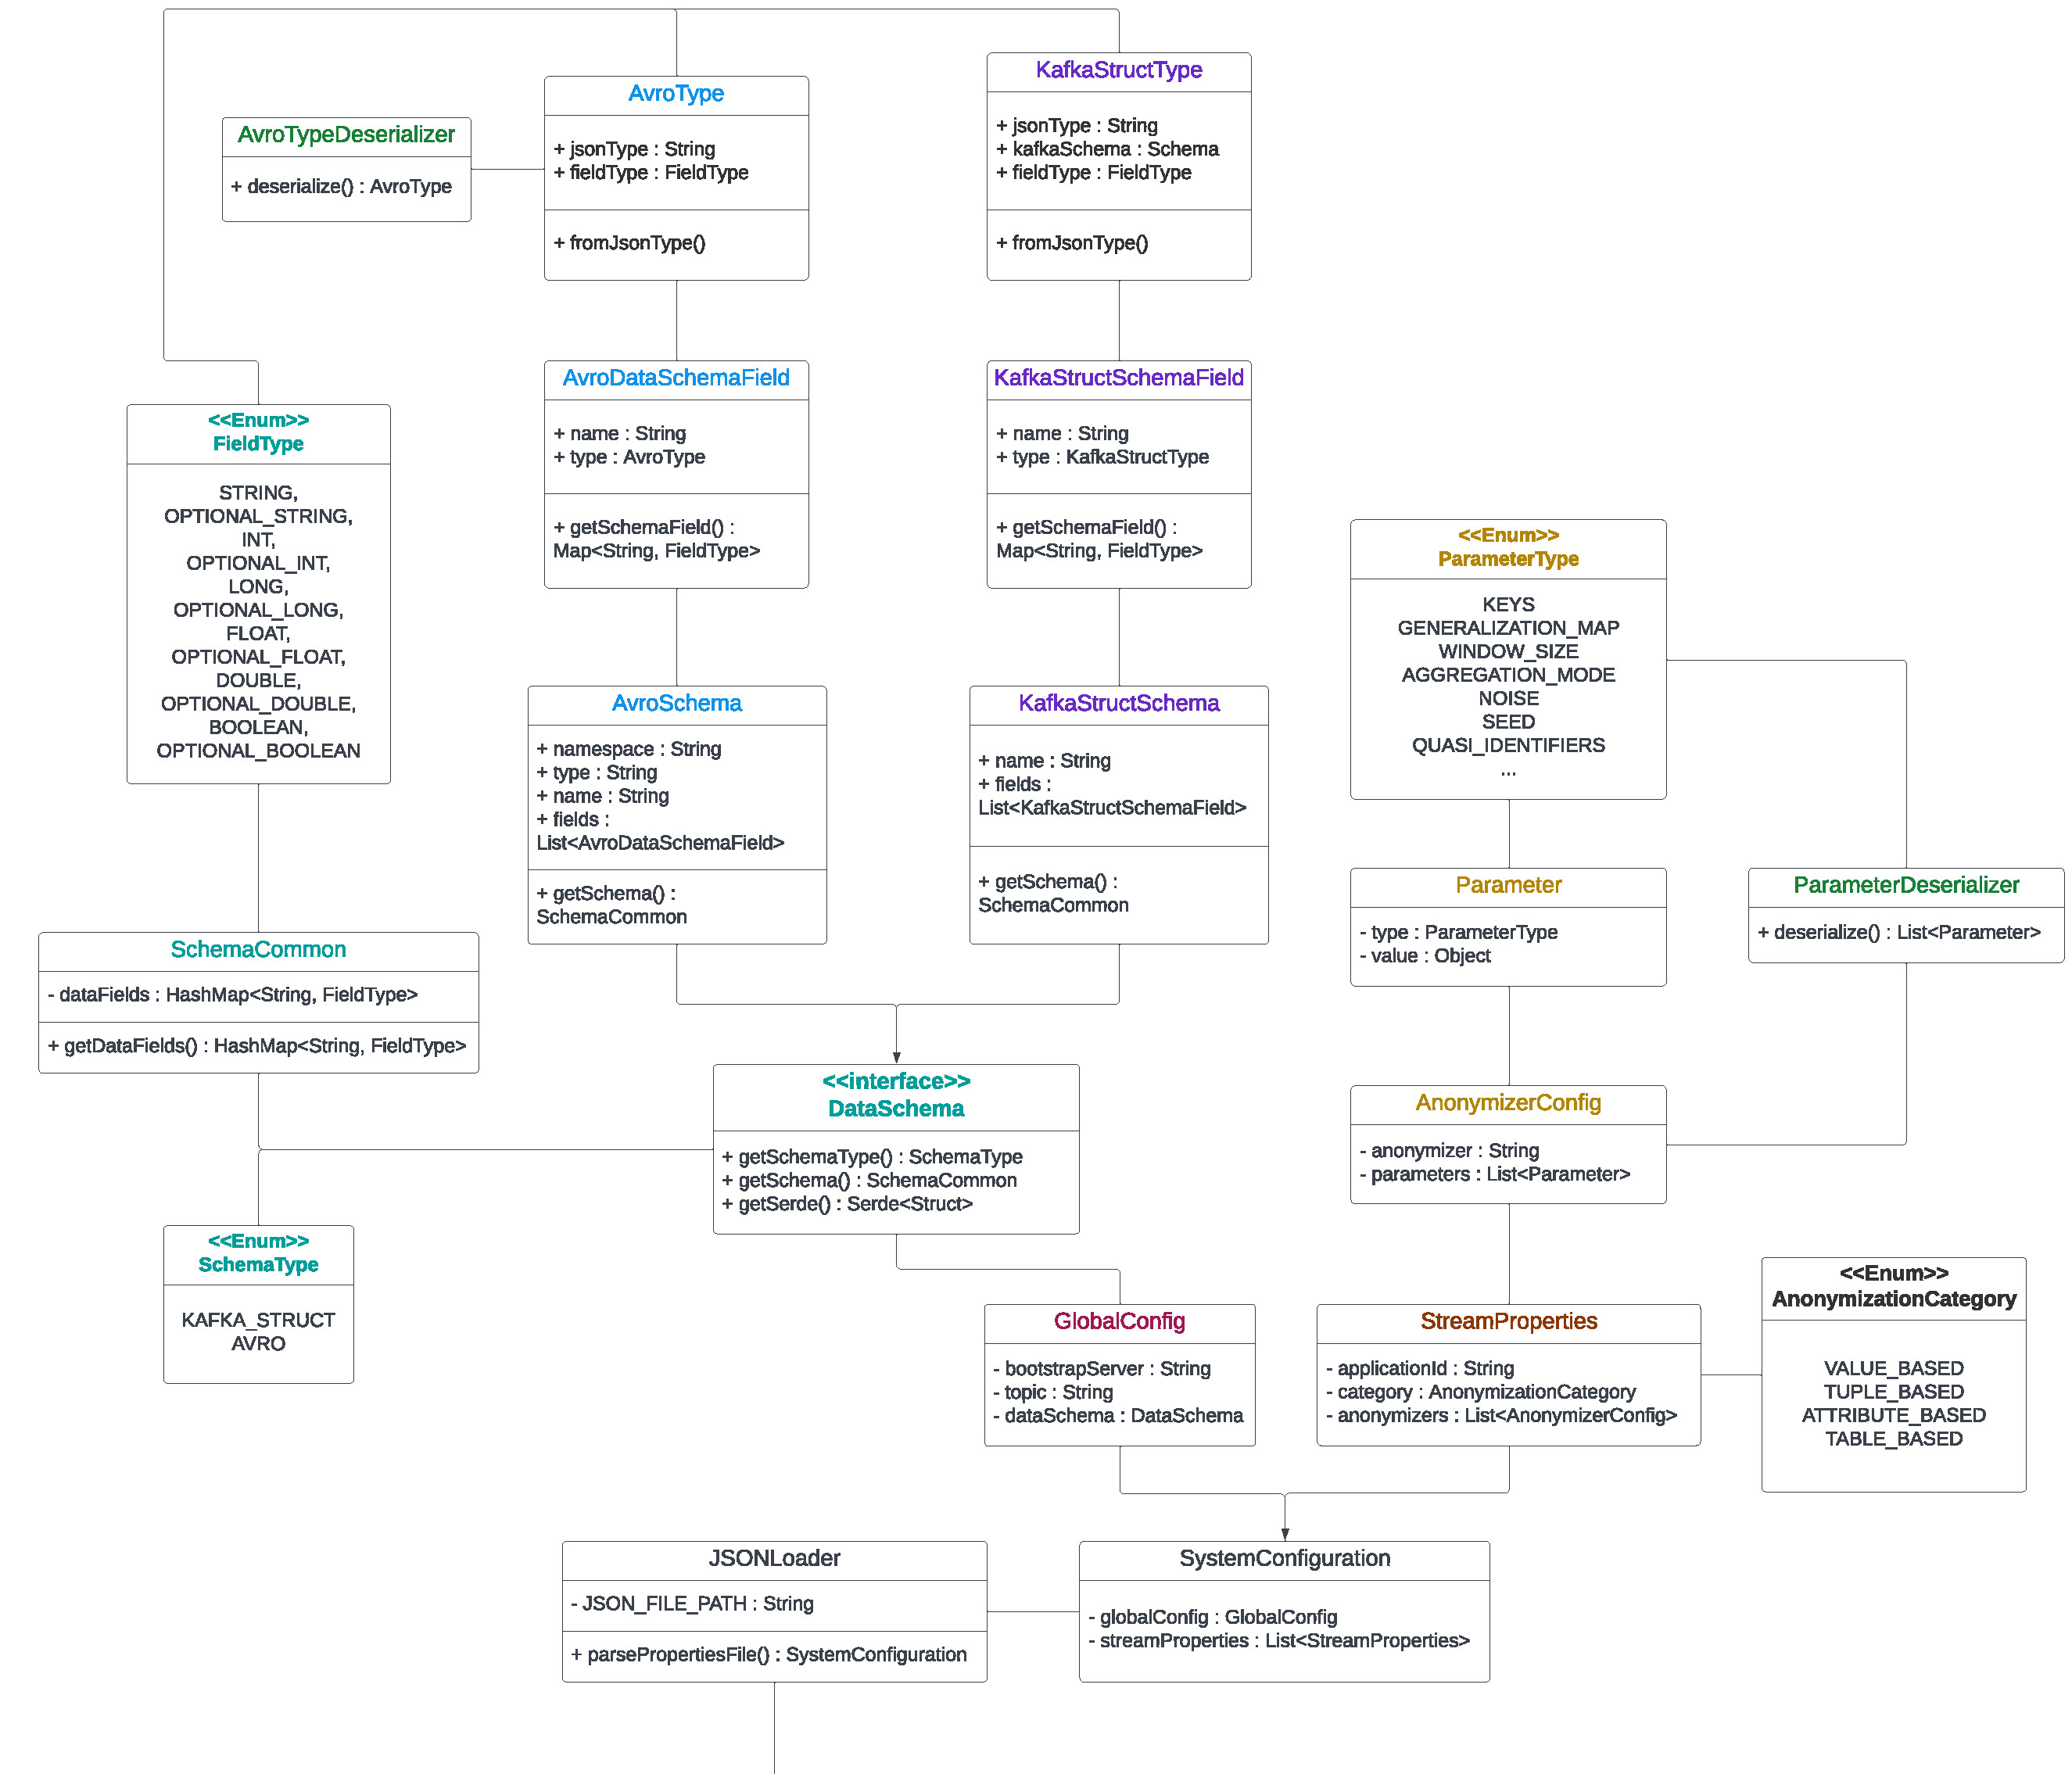
\includegraphics[width=0.85\pdfpagewidth]{img/Requirements_Parser_Class_Diagram.pdf}
   \end{adjustbox}
   \caption[Class diagram of the requirements parsing component of \ac{DASH}]{Class diagram of the JSON Loader responsible for parser the Data Officer's requirements. It connects on the bottom to the rest of \ac{DASH}. The full diagram can be found in the Appendix in Figure \ref{fig:full_class_diagram}\label{fig:requirements_parser}}
\end{figure}

Next to the \texttt{GlobalConfig} are the \texttt{StreamProperties}. Each stream includes at least one anonymizer. An anonymizer (highlighted in yellow) is specified with a name and its parameters. All available parameters of all anonymizers are represented as a constant in the \texttt{ParameterType} enum. As one anonymizer can include many parameters of different types a special \\ \texttt{ParameterDeserializer} was implemented. This deserializer processes each parameter in the list individually, converting it into an object as defined by the Parameter class corresponding to that ParameterType. These include simple types like double or int, but can simultaneously be more complex as hierarchies, enums, hashmaps, and lists. Again, \ac{DASH} has been designed to facilitate change. Adding new Parameters is as simple as adding a new value to the ParameterType enum and implementing its deserialization in the \texttt{ParameterDeserializer}.\par
The deserialization relies heavily on the correct format of the requirements and thus provides extensive error messages to the user, the Data Officer, upon failures. Additionally, a recipe with examples as well as documentation - is included in the artifacts found in the thesis repository (\url{https://github.com/TheRealHenri/master_thesis}). Consequently, the \texttt{JSONLoader} accomplishes another crucial task alongside the processing of the configuration, it checks the syntax of the requirements JSON. The deserialization accepts only the expected types for all classes and parameters. A wrong input syntactically will be caught here. The semantics of the requirements, specifically of the parameters, are validated in another component of \ac{DASH} responsible, which we will turn our attention to next. 

\subsection{Stream Config Validation and Construction\label{sec:config_builder}}
The \texttt{Stream Config Validation and Construction} aspect of DASH serves a fundamental role in preparing stream data for Kafka. It starts by taking \\ \texttt{StreamProperties} and methodically converting them into a Kafka-compatible configuration. This step involves not just creating configurations but also ensuring that each anonymizer's parameters undergo a strict validation process before they are used. The accompanying Class Diagram, shown in Figure \ref{fig:stream_config_builder}, outlines this essential process, with the functionality responsible for validation marked in teal and the functionality responsible for construction marked in red. \par

The central component is the \texttt{AnonymizationStreamConfigBuilder}, shown on the left in the figure. Algorithm \ref{algo:buildAnonymizationStreamConfig} shows pseudocode for its one method - \texttt{build(streamProperties)}. 

\begin{algorithm}[ht]
   \SetAlgoLined
   \SetKwInOut{Parameter}{Parameter}
   \SetKwInOut{Output}{Output}
   \Parameter{StreamProperties}
   \Output{Configuration for Kafka Streams}
   
   Validate StreamProperties \\
   
   \( anonymizationCategory \) ← null \\
   \( anonymizers \) ← Instantiate Anonymizers \\
   \ForEach{anonymizer}{
      \eIf{anonymizationCategory == null}{
         \( anonymizationCategory \) ← \( anonymizer \)'s anonymization category \\
      }{
         Validate \( anonymizationCategory \) \\
      }
      \( parameterExpectations \) ← \( anonymizer \)'s parameter expectations \\
      \ForEach{parameterExpectation}{
         \( parameterValidators \) ← \( parameterExpectation \)'s validators \\
         \ForEach{validator}{
            Validate Parameter
         }
      }
   }
   Initialize Anonymizers with their validated parameters\\

   \If{anonymizationCategory == ATTRIBUTE\_BASED}{
      Validate WindowConfig
   }

   \Return{new AnonymizationStreamConfig with Application ID, anonymizers list, and anonymizationCategory} \\
   \caption{Pseudocode for Building Stream Configurations}
   \label{algo:buildAnonymizationStreamConfig}
\end{algorithm}

The config builder first validates the input \texttt{StreamProperties} by checking whether an application ID for the stream is set and that it does not contain characters that Kafka does not allow i.e. spaces and other special characters. It also checks whether the specified anonymizers are available by verifying against the \texttt{AnonymizerRegistry}. The \texttt{AnonymizerRegistry} contains a map of all anonymizer names and corresponding anonymizer classes that are currently available in \ac{DASH}. \par
Next, the appropriate anonymizer class is instantiated. This is necessary to access their individual \texttt{getParameterExpectations}. For every parameter that an anonymizer offers, a \texttt{getParameterExpectation} is specified. It contains the parameter name, the validation logic and whether is it required for this anonymizer's functionality. The validation logic is encapsulated in a list of validators implementing the \texttt{ParameterValidator} interface. There are currently five validators for all the parameters used in \ac{DASH}, \texttt{KeyValidator}, \texttt{PositiveNumberValidator}, \texttt{QIKeysValidator}, \texttt{ConditionMapValidator} and an \texttt{EnumValidator}. \par 
To facilitate the validation the \texttt{AnonymizationStreamConfigBuilder} is instantiated with the \texttt{SchemaCommon} containing the data fields of the data schema of the underlying stream. For example, every single anonymizer requires a 'keys' parameter, which specifies the scope of the anonymizer's anonymize function. All attributes for a tuple with a key within the 'keys' parameter will get anonymized. A 'keys' parameter, therefore, is valid if there is an attribute in the data stream for every key. After the anonymizers are instantiated and their parameters are validated, they are initialized with their parameters. 

\begin{figure}[H]
   \begin{adjustbox}{center}
   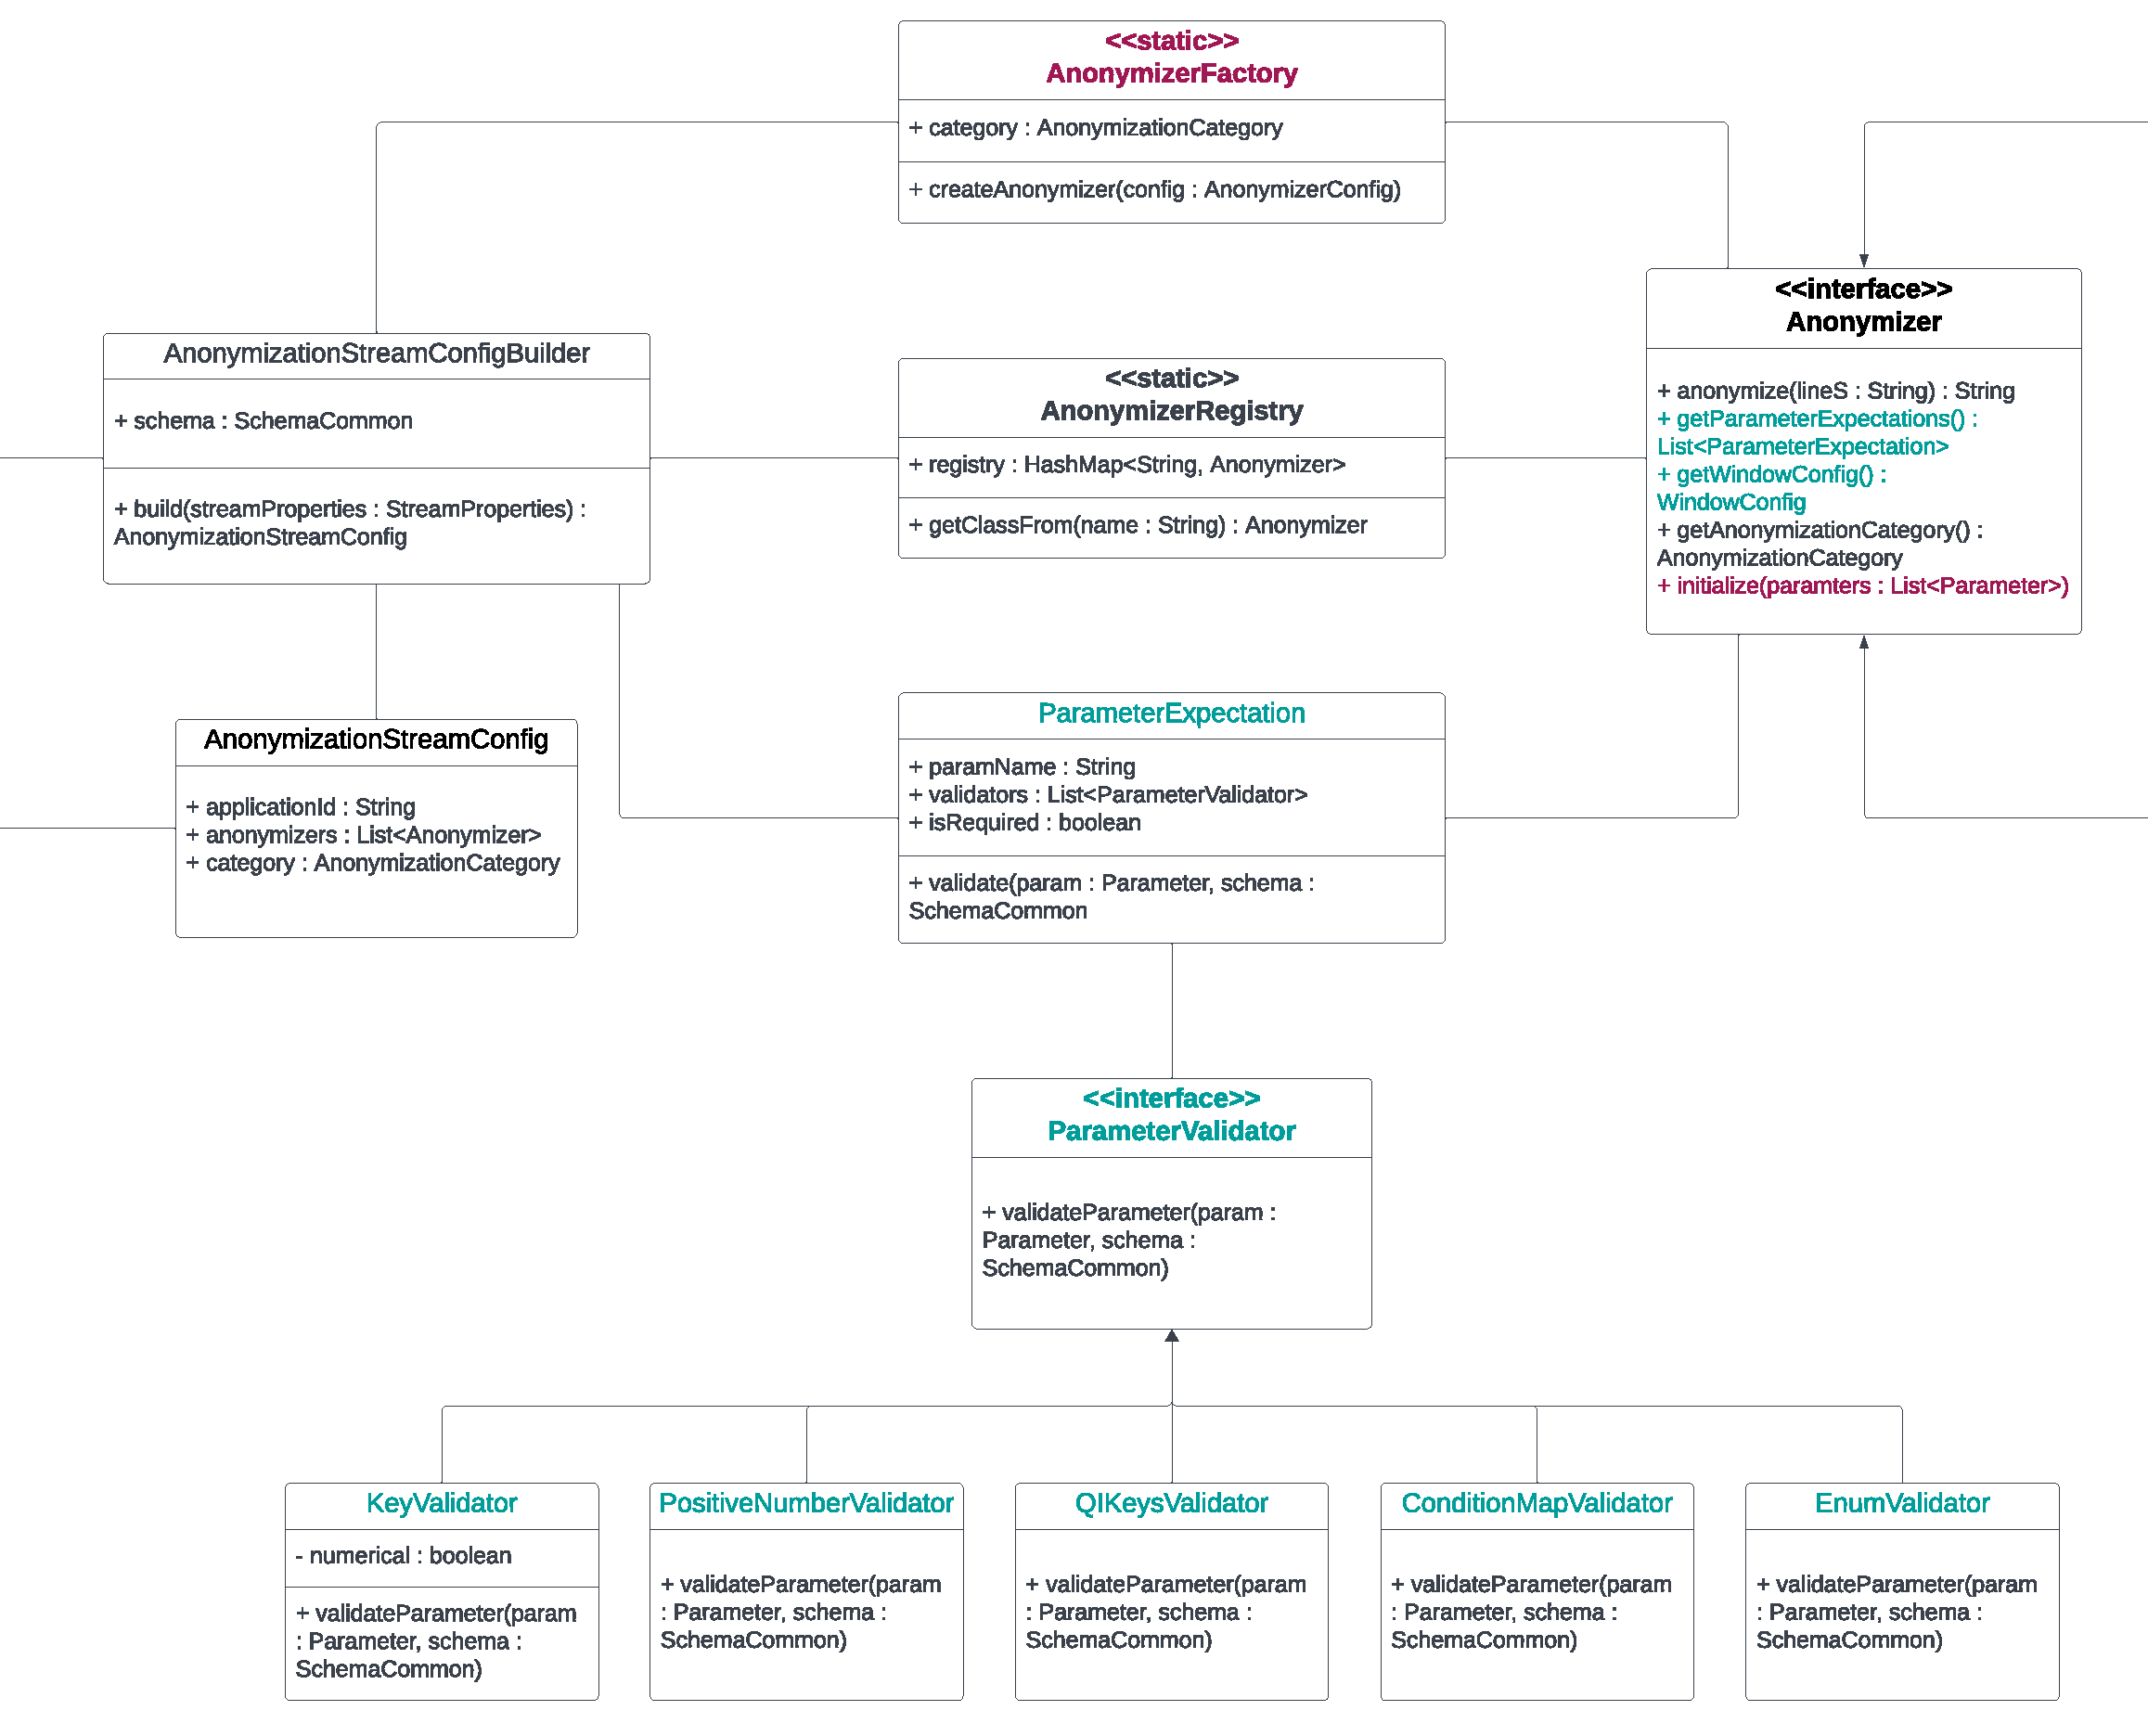
\includegraphics[width=0.85\pdfpagewidth]{img/Stream_Config_Builder.pdf}
   \end{adjustbox}
   \caption[Class diagram of the configuration builder component of \ac{DASH}]{Class Diagram of the stream configuration builder component and its corroborators responsible for validating (highlighted in teal) and instantiating (highlighted in red) individual anonymization stream configurations. It connects on the right to the individual anonymizers and on the left to the managing component of \ac{DASH}. The full diagram can be found in the Appendix in Figure \ref{fig:full_class_diagram}\label{fig:stream_config_builder}}
\end{figure}

Following the initialization, for an anonymization stream with attribute-based anonymizers their windowing strategy is validated. As many anonymizers can be included in one stream, but only one windowing technique is applied per stream, it must be ensured that all anonymizers have the same window configuration. \par
Finally, a new \texttt{AnonymizationStreamConfig} is created and returned, which includes the stream's name, its anonymizers, and the anonymization category. \par
If any of these validations fail \ac{DASH} will not proceed to running any streams, instead the setup phase will fail and an extensive log is output to the Data Officer to aid in fixing the setup mistakes. 

\subsection{Centralizing Stream Management\label{sec:stream_manager}}
The \texttt{StreamManager} functions as the operational extension of the Data Officer within \ac{DASH}. This entity centralizes all operations and handles both internal and external communications within \ac{DASH}. Take a look at Figure \ref{fig:stream_manager} for the Class Diagram. In the diagram, all green highlighted functionalities are directly administrable by the Data Officer. 

\begin{figure}[ht]
   \begin{adjustbox}{center}
      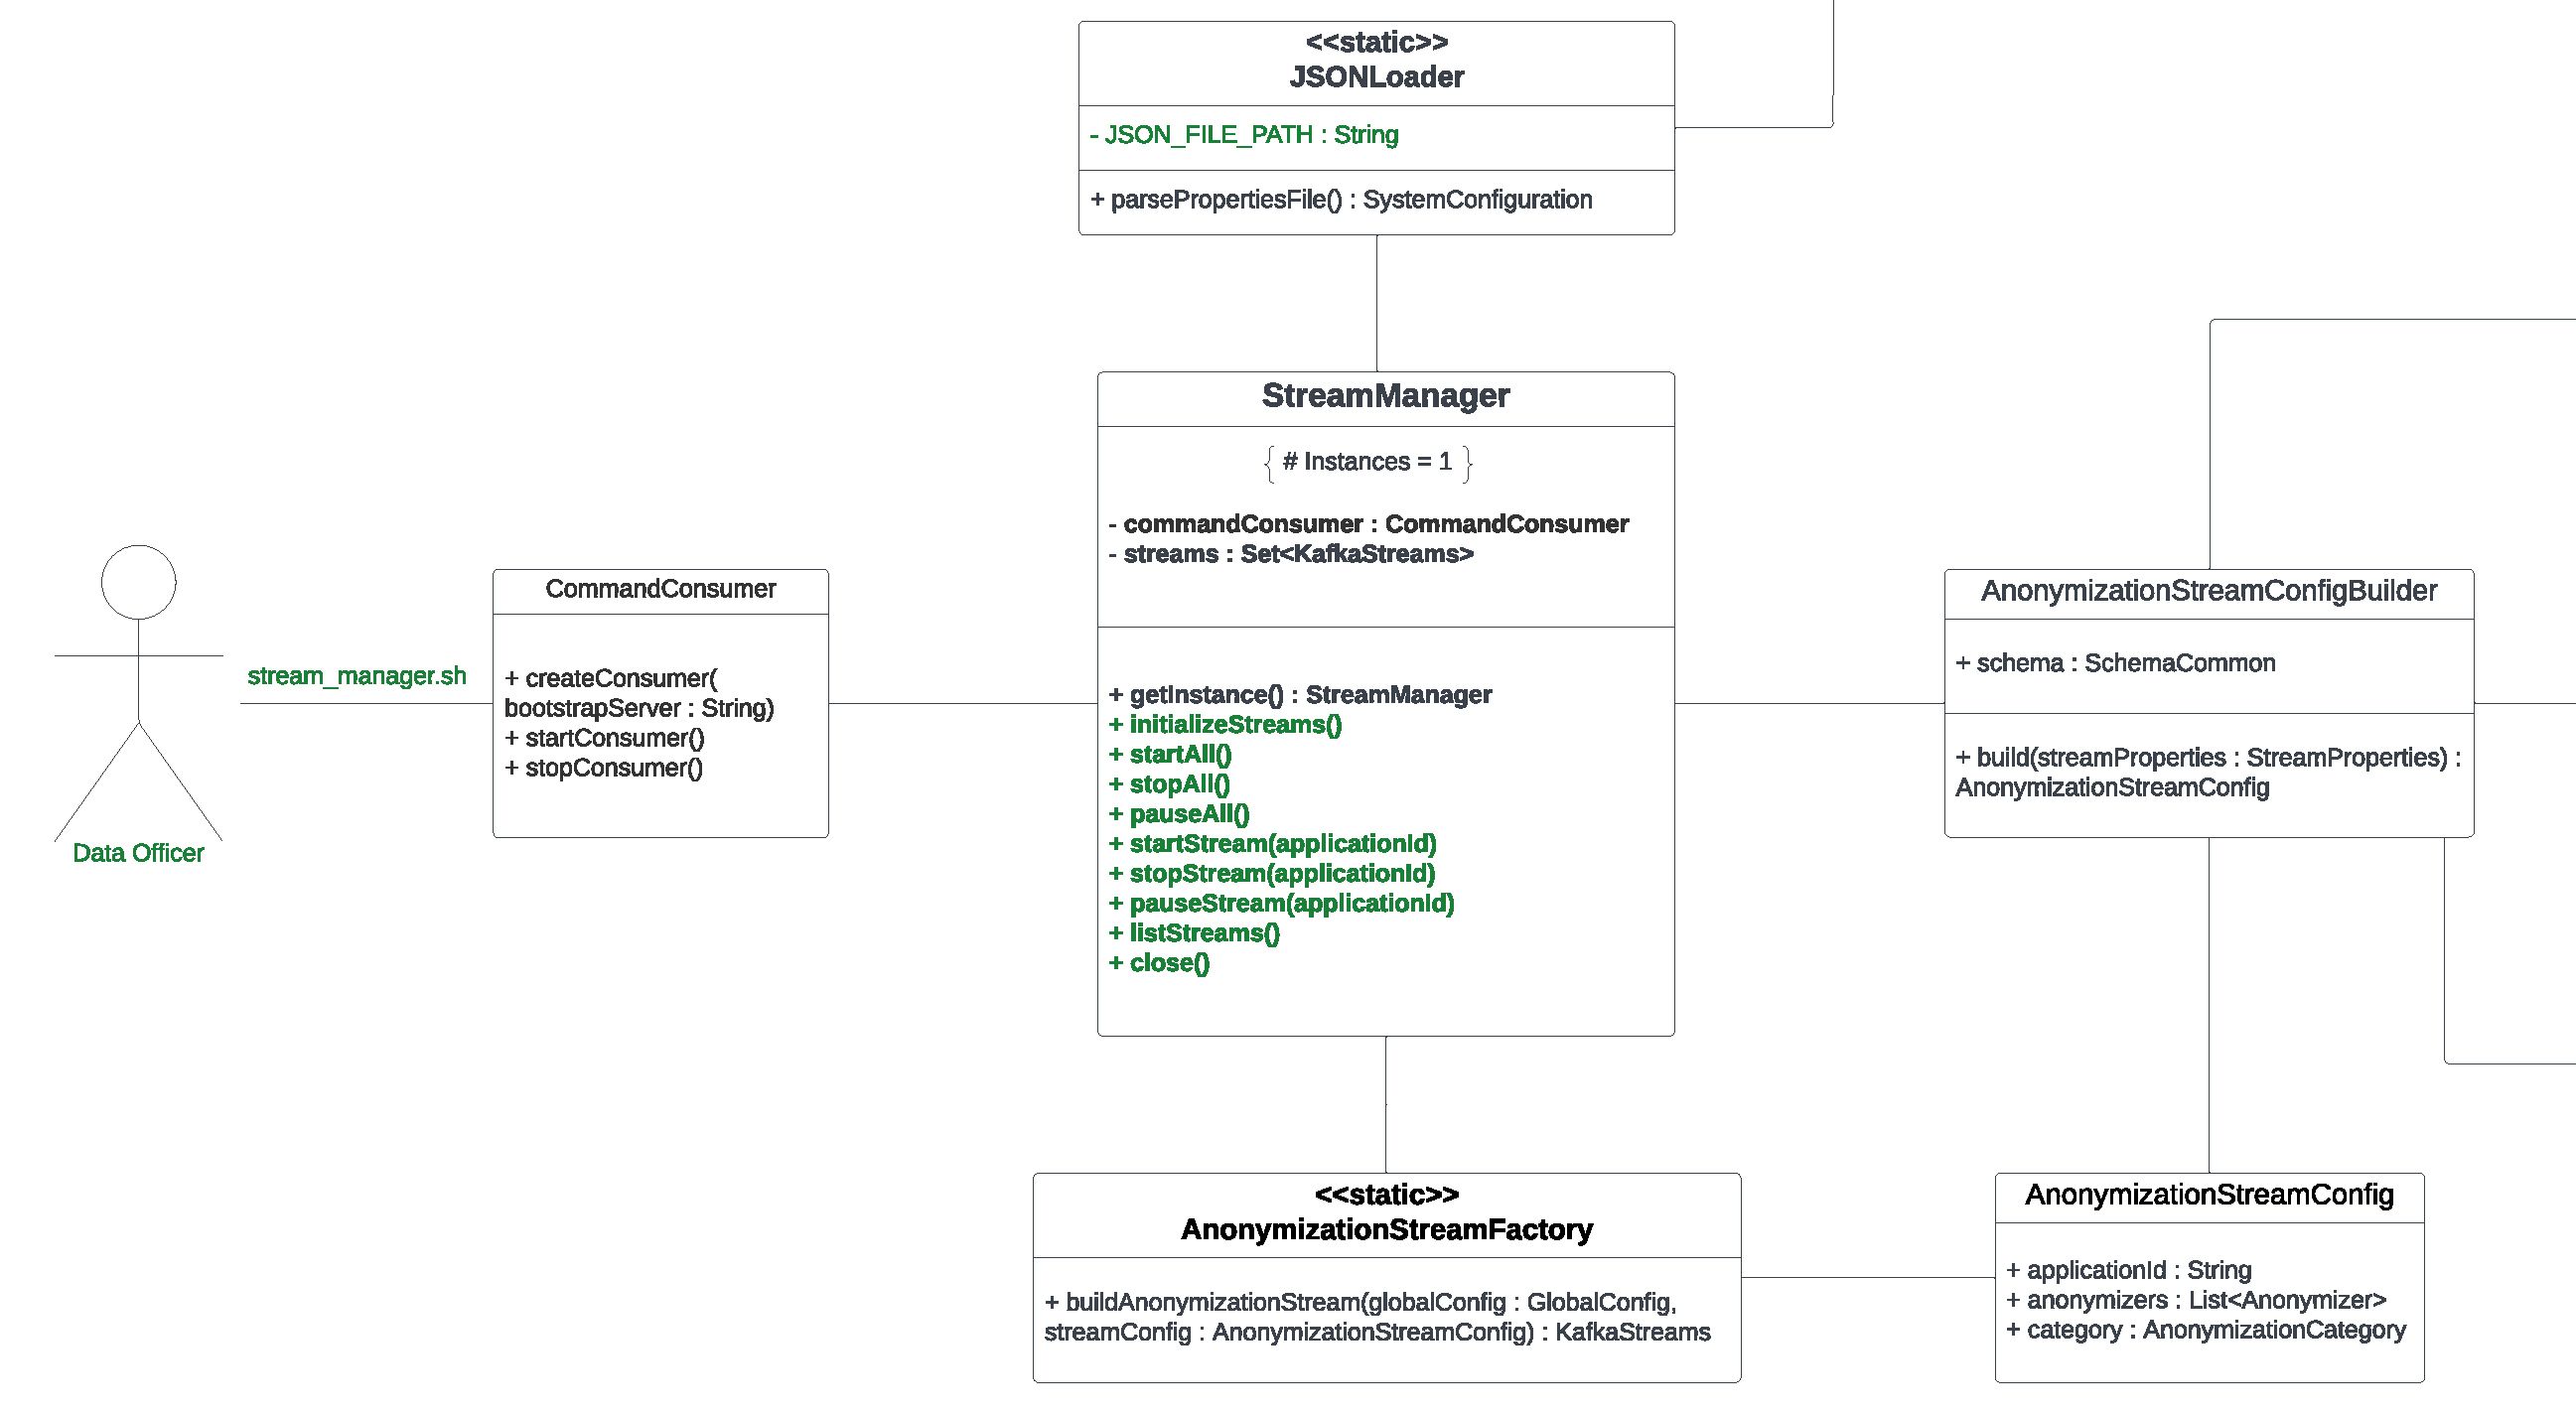
\includegraphics[width=0.85\pdfpagewidth]{img/Stream_Manager.pdf}
      \end{adjustbox}
      \caption{The central component of DASH illustrated in a UML Class Diagram. All green highlighted functionalities are directly administered by the Data Officer. It connects at the top to the rest of the requirements parsing component, and to the right to the stream configuration building component. The full diagram can be found in the Appendix in Figure \ref{fig:full_class_diagram}\label{fig:stream_manager}}
\end{figure}

In the center is the \texttt{StreamManager}. The constraint notation beneath the class name in Figure \ref{fig:stream_manager} denotes the Singleton pattern, ensuring a single instance is instantiated and globally accessible within the system. The Data Officer invokes system actions through the \texttt{stream\_manager.sh} shell script, located at the system's root directory. This opens up a command line, which internally creates (in true Kafkaesque fashion) a Kafka Producer. Commands issued during the session are produced to a designated 'commands' topic. The CommandConsumer within DASH subscribes to this topic and forwards the commands to the StreamManager. The commands encompass initialization, starting, pausing, and stopping of all or individual streams, and terminating \ac{DASH}. Additionally, there is a help command, which is also invoked on wrong input, to aid the Data Officer in administering and a list command to monitor the running system.
The \texttt{JSONLoader} as well as the \texttt{AnonymizationStreamConfigBuilder} and the \texttt{AnonymizationStreamConfig} are previously introduced components, serving specific functions in stream configuration and setup. The \texttt{AnonymizationStreamFactory} handles the creation and configuration of the anonymization streams on the Kafka side. The global config defines the source Kafka Stream. The tuples then are forwarded to the stream specified in the \texttt{AnonymizationStreamConfig}. Subsequently, tuples are anonymized according to their category, as determined by the configuration. The anonymization itself is executed by the function within the anonymizer, which is specified by the configuration. In the case of an attribute-based stream, the stream is first windowed according to the specification, aggregated, and then forwarded as a collection of tuples to the anonymizers. All streams can contain multiple anonymizers, which process the data sequentially. This means that the output of the first anonymizer will be the input of the second anonymizer and so on.\par
Ultimately, the system publishes the anonymized tuples to a newly created topic within Kafka. Its naming convention is '\{source\_stream\_name\}-\{application\_id\}'. From here they exist in the Kafka server and can be consumed from outside \ac{DASH}. In combination with the aforementioned RBAC system, these newly produced topics can be restricted to be only consumable by users who are assigned to a certain role. 

\section{Data Pipeline}
To facilitate the development and evaluation of \ac{DASH} and \ac{RBAC} mechanisms within Kafka, we implemented a data pipeline. It encompasses a data generator feeding data into a custom Kafka Connector. Within Kafka, the data is anoynmized and distributed into multiple role-restricted output data streams. These are read by Kafka Consumers. Figure \ref{fig:data_pipeline} depicts the flow of data from the source to the destination as indicated by the blue arrows. Each component is associated with its respective detailed explanation in the indicated sections. 

\begin{figure}[ht]
   \begin{tikzpicture}[node distance=2.3cm, auto, trim left=-0.25cm]
      \tikzstyle{system} = [rectangle, draw, rounded corners, text width=5em, text centered, minimum height=3em]
      \tikzstyle{arrow} = [thick,->,>=stealth]

      \node [system] (datagen) {Data Generator};
      \node [system, right=of datagen] (kafkacon) {Kafka Connector};
      \node [system, right=of kafkacon] (Kafka) {Kafka};
      \node [system, right=of Kafka] (kafkacons) {Kafka Consumers};

      \draw [arrow, color=dataBlue] (datagen) -- node[anchor=south] {\footnotesize{CSV data}} (kafkacon);
      \draw [arrow, color=dataBlue] (kafkacon) -- node[anchor=south] {\footnotesize{Struct data}} (Kafka);
      \draw [arrow, color=dataBlue] (Kafka) -- node[anchor=south, text width=2cm, text centered] {\footnotesize{Anonymized \\ structs}} (kafkacons);

      \node [above of=datagen, yshift=-0.5cm] (sec1) {Section \ref{sec:data_gen}};
      \node [above of=kafkacon, yshift=-0.5cm] (sec2) {Section \ref{sec:kafka_connector}};
      \node [above of=Kafka, yshift=-0.5cm] (sec3) {Section \ref{sec:dash}};
      \node [above of=kafkacons, yshift=-0.5cm] (sec4) {Section \ref{sec:kafka_consumer}};
      
      \draw [<-, color=black, dashed] (datagen.north) -- (sec1);
      \draw [<-, color=black, dashed] (kafkacon.north) -- (sec2);
      \draw [<-, color=black, dashed] (Kafka.north) -- (sec3);
      \draw [<-, color=black, dashed] (kafkacons.north) -- (sec4);
\end{tikzpicture}
\caption{Data Pipeline of the Implementation: The diagram shows the various components and their data flow, indicated by blue arrows, with references to the corresponding sections.}
\label{fig:data_pipeline}
\end{figure}
   
In this section, we will take a closer look at the components of the data pipeline outside of Kafka. It follows the flow of data beginning with the generator. 

\subsection{Data Generator\label{sec:data_gen}}
The data generator, developed in Python and accessible via a Jupyter Notebook \cite{jupyter_notebook}, is designed to simulate patient data for a German hospital specializing in diabetes care, as detailed in the Use Case Example (Section \ref{sec:anon_granularity}). Operating on a Python3 kernel, this generator utilizes modules such as Pandas \cite{pandas}, Numpy \cite{numpy}, and Faker \cite{faker} to create and manipulate CSV data. \par
The number of lines generated can be specified at the top of Data Generation section of the \texttt{dataGenerator.ipynb} notebook by adjusting the \texttt{nRows} value. A sample collection of data generated in this way with $nRows = 40$ is shown in the Appendix in Table \ref{tab:patient_data}. The script employs the Faker module for generating realistic yet fictitious personal data, such as names, addresses, and phone numbers. Additionally, a seed can be specified to easily reproduce the same data. \par
The data generator also ensures diversity in data by assigning gender, diagnosis, insurance companies, and other patient attributes based on realistic distributions and correlations. For instance, the genders Male and Female are assigned 48 percent of the time respectively for each entry, and 2 percent it assigned to Non-Binary. Similarly, it generates the diagnosis of Type 1 in nine percent of the cases, Type 2 in 89 percent, and Type 1.5 in the remaining two. An insurance company is randomly assigned to each entry according to their distribution in Germany. Height, weight, age, glucose, and HbA1C are randomly assigned from within a provided reasonable range. The medication is correlated with the diagnosis. \par
The generator's design allows for straightforward adjustments of data randomness, structure, and volume, which can be configured in the initial cell of the notebook.

\subsection{Kafka Connector\label{sec:kafka_connector}}
Since CSV files cannot be directly published to the Kafka network, it requires the use of a middleman, a Kafka Producer. This requirement is frequently encountered by Kafka users. This is where Kafka Connectors come into play. They alleviate this task of developing a Producer manually and transform the data for the user. There are many such Connectors available, but most are restricted by licenses that restrict their usage. Therefore, we developed our own Kafka Connector for CSV files. \par
Implementing a custom connector involves utilizing two key interfaces of the Kafka Connect framework: \texttt{SourceConnector} and \texttt{SourceTask}. The source connector class sets up the connection to Kafka. This includes setting the properties for the server, the security protocols, and the topic name that the connector should produce to. It also specifies the \texttt{SourceTask} class and how many instances of that class should run simultaneously.\par
The implemented task reads the CSV file located in a fixed location. Data is read into a buffer employing Java's \texttt{BufferedReader}. This buffer, containing a batch of lines, is then processed. Lines are extracted by detecting end-of-line characters '$\backslash$n' and '$\backslash$r'. The lines are converted into Kafka Structs with a predefined Schema that fits the data generated by the aforementioned Python script. Ultimately, the structs are produced to the specified topic in batches. \par
The connector is integrated with the Kafka server by compiling the Java code into a JAR file and transferring this file to Kafka's distribution data folder. Subsequently, it can be executed with the specified properties at runtime.

\subsection{Kafka Consumers\label{sec:kafka_consumer}}
In general, the terminal consumers included in the Apache Kafka distribution suffice for numerous implementations. It simply consumes the tuples from a specified topic. However, when implementing access control and simultaneously monitoring multiple data streams, the setup becomes laborious. \par
Consequently, a script was developed to instantiate consumers with predefined roles, including authentication, in a unified setup. It is set up with the specifications of the default \ac{DASH} configuration and writes the consumed tuples to the terminal. Unlike default terminal consumers that output data as plain text, custom consumers recognize the data structure and display it in a more aesthetically pleasing format. \par
The implementation details are available in the 'consumers' folder within the Kafka pipeline directory.


\section{Docker-based System Integration}
The systems developed, including Kafka, ZooKeeper, the \ac{RBAC} system, \ac{DASH}, the data generator, the source connector, and consumers, are designed to operate in conjunction. This ensemble forms a complete data pipeline, simulating data streams being anonymized in real-time. However, the simultaneous management of seven or more systems can be a fault-prone and tedious process, requiring the handling of numerous terminals and configurations. This is why we have opted early in the development process to unify building, deploying, and running all systems in containers using Docker \cite{docker}. \par
Docker facilitates the containerization of applications into standardized, executable components. This is achieved by allocating resources from the underlying hardware for use by the Docker engine. Atop this engine, within the container, developers can freely choose the operating system to build the application. The application within the container will then be runnable on any environment simplifying the deployment. \par
The integration of multiple containers is efficiently achieved through a 'Docker Compose' file. Each Docker container is specified as a service in the compose file. This is how our systems are unified and become executable in any environment with the simple command \texttt{Docker compose up} in the code folder of the repository (which can be found alongside all other artifacts, the thesis itself, and relevant literature in \url{https://github.com/TheRealHenri/master_thesis}).\par
The compose file is written in yaml and lists services e.g. containers followed by internal structures such as networks and Docker volumes. The latter can be used for persisting storage generated by and used by Docker containers. There are two types of volume storage: bind mounts point to the storage of the host system, Docker volumes on the other hand are completely managed by Docker. 
Each service represents a Docker container and consists of its specifications as shown in Code Fragment \ref{lst:docker_container}. 

\begin{lstlisting}[language=yaml, captionpos=b, caption={General structure of a docker compose file.}, label={lst:docker_container}]
   service_name:
      build: ./path/to/project 
      # alternatively: 
      image: 'dockerhub_link'
      networks:
         - network_name
      ports: 
         - internal_port:exposed_port
      depends_on:
         - other_service_name
      environment: 
         - variable_name: variable_value
      volumes: 
         - ./storage/path/locally:/docker/path1
         - docker-volume:/docker/path2
      command: executed_on_startup
   
   other_service_name: 
      ...
   
   networks: 
      network_name: 
         driver: driver_type
   
   volumes: 
      docker-volume:
\end{lstlisting}
   
For each service within Docker, the specification of either a build or an image is mandatory. The build refers to a project with its own Dockerfile. Images may be selected from Docker Hub \cite{dockerhub}. We use the \texttt{bitnami/zookeeper:3.8.2} image for zookeeper and the \texttt{bitnami/kafka:3.5.1} image for kafka. The rest of our systems were developed from scratch and included a Dockerfile with the necessary build information. \par
In the docker compose, we specify a network for all containers to use called simply 'kafka\_network'. This allows containers within the network to communicate with each other by service name instead of IP address. In addition, communication necessitates exposed ports; without these, inter-container is not possible. Ports exposed by the application running inside a container need to be mapped to ports accessible from the outside. For instance, Kafka exposes the communication port 9092 to its clients and on port 8083 with its connectors. The communication between Kafka and Zookeeper occurs on port 2021. We have set up the data generator to run on a web socket on port 8888, so if someone using the system wants to change the way data is generated, the person can do it during runtime with a user interface in the browser at \texttt{localhost:8888}. \par
Dependencies among containers are also managed through the Docker Compose file. For instance \ac{RBAC}, \ac{DASH}, and the Kafka Connector are dependent on a running Kafka server. Kafka in turn is dependent on a running ZooKeeper instance. These dependencies can be specified by simply adding the name in the 'depends\_on' section of the compose. Furthermore, since version 3 of compose, the status of the dependent container can be specified as well. We require the data pipeline build process to be finished successfully before starting the Kafka connector. This better allocates resources at runtime by not spending it on processes that would have to wait for others later on. \par
Environment variables correspond to configuration parameters within the system. Commonly, there is a set of parameters available for images from Dockerhub. In the case of the Kafka image, several parameters have to be set. For one the listeners dictate the protocols used for internal and external communication with the server. Additionally, the zookeeper communication is specified as well. In our docker compose we emulate a distributed event store. For this, we run the Kafka server on three different brokers. Each broker is assigned its container, they differentiate in their port mappings as well as, crucially, their broker ID environment variable. All clients and connectors specify all three brokers as their bootstrap server e.g. \texttt{bootstrapServer=kafka1:9092,kafka2:9093,kafka3:9094}. \par
We utilize Docker volumes for data storage. As intended by Docker we use bind mounts for data we specify on the host system like the Data Officer's anonymization requirements, Kafka Connector's configuration, and the \ac{RBAC} database. For data shared between containers, we use specific Docker volumes managed by Docker. For example, the data generator produces a CSV file used by the Kafka Connector. Produced logs are also stored in Docker. \par
Finally, a command can be specified to be executed upon completion of the build process. Calling \texttt{docker compose up} starts up all containers and executes the specified command. The \ac{RBAC} system opens a shell for the \ac{CLI}, while the Kafka Connector is started up with a shell script. \par
Ultimately, Docker is configured to initially launch ZooKeeper, followed by the Kafka server with three operational brokers for load balancing. In the meantime, data is generated. Upon completion, the Kafka Connector, the \ac{RBAC} system, and \ac{DASH}. The generated data is fed through the Connector into \ac{DASH} and produced to the anonymized streams. This entire process is executable through a single command in one terminal, provided Docker is installed on the host system. 
    \chapter{Testing and Evaluation\label{cha:chapter5}}
In the thesis 

\section{Experimental Setup\label{sec:exp}}
... should include the following:
\begin{itemize}

\item define experimental data and workload(s),
\item discussion about the selection and interpretation of the evaluation metrics,
\item discussion about the computing environment, including hardware, software, and tools.
\end{itemize}

\subsection{Experimental Design}

Tuple-based perform exceptionally well and are well-suited in data streaming. Essentially  no latency and no considerable overhead in throughput. 

Aggregation is another topic altogether. 


\section{Parameter Optimization\label{sec:parameterOptimization}}


\subsection{Interpretation of the Results}
This sub-section should include
\begin{itemize}
\item description and an interpretation of the experimental results.
\item explanation for any anomalies or any unexpected behavior.
\end{itemize}


    \chapter{Conclusion\label{cha:chapter6}}

\section{Future Work}

... should include the following:
\begin{itemize}

\item problem restated and a brief summary of the methodology,
\item student contributions (e.g., survey, open-source software, journal publication),
\item a brief summary of the findings and results,
\item limitations and generalizability of the findings and results.
\item lessons learned,
\item recommendations for future research.

\end{itemize}



% ---------------------------------------------------------------

%Bibliography
\begingroup
\raggedright
\bibliographystyle{splncs03}
%\bibliographystyle{acm}
\bibliography{bibliography, mendeley_library}
\endgroup

%appendix
\addchap{Appendix A. Further Details on the Solution Approach\label{app:A}}

\begin{sidewaystable}
    \centering
    \tiny
    \begin{longtable}{lllllllllllllll}
        \caption{Extended table of patient data used. The table shows a part of the data used when testing the system. The attribute abbreviations correspond as follows: hgt - height; wgt - weight; ins.\_company - insurance\_company; ins.\_number - insurance\_number, diag. - diagnosis; gluc. - glucose.} \label{tab:patient_data}\\
    \toprule
    \textbf{id} & \textbf{name} & \textbf{address} & \textbf{zip} & \textbf{phone} & \textbf{gender} & \textbf{hgt} & \textbf{wgt} & \textbf{age} & \textbf{ins.\_company} & \textbf{ins.\_number} & \textbf{diag.} & \textbf{gluc.} & \textbf{hba1c} & \textbf{medication} \\
    \midrule
    \endfirsthead
    
    \multicolumn{15}{c}%
    {{\tablename\ \thetable{} -- continued from previous page}} \\
    \toprule
    \textbf{id} & \textbf{name} & \textbf{address} & \textbf{zip} & \textbf{phone} & \textbf{gender} & \textbf{hgt} & \textbf{wgt} & \textbf{age} & \textbf{ins.\_company} & \textbf{ins.\_number} & \textbf{diag.} & \textbf{gluc.} & \textbf{hba1c} & \textbf{medication} \\
    \midrule
    \endhead
    
    \bottomrule
    \endfoot
    
    \bottomrule
    \endlastfoot
    
    
    1 & Sarah Kreusel & Benthinring 6 & 34597 & 0711 98 81331 & Female & 169 & 62 & 95 & 108312586 & L660487647 & E11 & 65 & 9.36 & Metformin \\
    2 & Ronny Kohl & Sauerplatz 42 & 93801 & 089 14407487 & Male & 180 & 73 & 68 & 103508742 & R938242194 & E11 & 157 & 7.77 & Metformin \\
    3 & Lilly Geißler & Mühlestr. 565 & 66369 & 03525914827 & Female & 170 & 51 & 75 & 108928697 & B659387784 & E11 & 98 & 9.79 & Metformin \\
    4 & Marian Bauer & Bruderweg 6/2 & 27618 & 034 56379318 & Male & 189 & 69 & 23 & 103306961 & N988901370 & E10 & 112 & 8.67 & Insulin \\
    5 & Sandra Jähn & Södinggasse 82 & 87339 & 02437 40551 & Female & 166 & 64 & 61 & 101002659 & R453561328 & E10 & 382 & 8.88 & Insulin \\
    6 & Steffen Henk & Junkenallee 03 & 11517 & 03939818024 & Male & 169 & 82 & 57 & 103508742 & Z988986270 & E11 & 96 & 5.76 & Metformin \\
    7 & Dennis Dobes & Trübplatz 465 & 00839 & 08180041538 & Male & 178 & 94 & 86 & 109500490 & T577049432 & E11 & 437 & 7.8 & Metformin \\
    8 & Arif Geisler & Bienstraße 792 & 34510 & 09659 95631 & Diverse & 169 & 61 & 68 & 109500490 & Z210900364 & E10 & 182 & 5.6 & Insulin \\
    9 & Udo Bürger & Kunst Allee 3 & 44149 & 023 1977653 & Male & 182 & 92 & 61 & 109519176 & J339204213 & E11 & 179 & 7.7 & Metformin \\
    10 & Max Mustermann & Wegstr. 42 & 69840 & 0309 049397 & Male & 175 & 80 & 40 & 109500398 & E822232308 & E11 & 120 & 7.0 & Metformin \\
    11 & Erika Mustermann & Hauptstr. 5 & 52820 & 04839768544 & Female & 165 & 65 & 36 & 108817930 & K759451642 & E10 & 140 & 6.8 & Insulin \\
    12 & Julia Schmidt & Bergweg 13 & 33888 & 0612347192 & Female & 168 & 60 & 28 & 109000051 & L858268436 & E11 & 150 & 7.5 & Metformin \\
    13 & Tobias Müller & Seeallee 21 & 78151 & 07899 544559 & Male & 180 & 85 & 55 & 108928697 & I998139981 & E11 & 130 & 6.9 & Metformin \\
    14 & Christina Klein & Talweg 8 & 37111 & 0603328566 & Female & 160 & 55 & 33 & 108888888 & K926100157 & E10 & 135 & 7.2 & Insulin \\
    15 & Uwe Lehmann & Stadtweg 14 & 27417 & 04896 92775 & Male & 175 & 78 & 45 & 109500398 & P619653870 & E10 & 145 & 7.1 & Insulin \\
    16 & Anna Becker & Waldstr. 3 & 10044 & 08645 546756 & Female & 170 & 68 & 31 & 108312586 & D769681473 & E11 & 155 & 7.6 & Metformin \\
    17 & Frank Schubert & Blumenweg 7 & 19364 & 0087010395 & Male & 178 & 82 & 48 & 109500787 & G425120298 & E11 & 125 & 7.4 & Metformin \\
    18 & Kathrin Neumann & Feldstr. 11 & 56066 & 0759017707 & Female & 162 & 58 & 29 & 108814099 & L006897178 & E10 & 138 & 7.3 & Insulin \\
    19 & Lars Hoffmann & Wiesenweg 18 & 75261 & 06671 81305 & Male & 182 & 90 & 52 & 109000051 & A510337443 & E11 & 128 & 6.7 & Metformin \\
    20 & Sabine Fuchs & Bachstr. 22 & 68656 & 06366 46753 & Female & 167 & 63 & 34 & 109500398 & H758511496 & E10 & 132 & 7.0 & Insulin \\
    21 & Dirk Sommer & Forstweg 5 & 73277 & 09304 75332 & Male & 170 & 76 & 43 & 109500787 & M562343754 & E10 & 142 & 6.9 & Insulin \\
    22 & Marie Lange & Hügelstr. 9 & 72773 & 0353876928 & Female & 165 & 61 & 38 & 108313123 & D564564174 & E11 & 160 & 7.8 & Metformin \\
    23 & Oliver Krause & Grabenstr. 2 & 35141 & 01214338986 & Male & 180 & 84 & 50 & 101002659 & U921658735 & E11 & 118 & 6.8 & Metformin \\
    24 & Susanne Winter & Brunnenweg 19 & 01870 & 05033 36428 & Female & 159 & 54 & 32 & 108918320 & Q667879936 & E10 & 137 & 7.1 & Insulin \\
    25 & Markus Winkler & Kanalweg 4 & 90111 & 06309 336421 & Male & 176 & 77 & 46 & 103306961 & X360906143 & E10 & 148 & 7.0 & Insulin \\
    26 & Stefanie Berger & Bahnhofstr. 31 & 83716 & 0371472504 & Female & 169 & 67 & 39 & 108811215 & I955572981 & E11 & 153 & 7.7 & Metformin \\
    27 & Peter Klein & Rosenweg 12 & 30962 & 01556 031663 & Male & 179 & 83 & 51 & 109500398 & H607086736 & E11 & 121 & 6.6 & Metformin \\
    28 & Claudia Schmitt & Kirchweg 29 & 57024 & 09251 652740 & Female & 164 & 59 & 30 & 101575519 & T477237457 & E10 & 136 & 7.2 & Insulin \\
    29 & Heiko Schulz & Sonnenallee 23 & 67294 & 07686863295 & Male & 183 & 88 & 53 & 108928697 & K281348102 & E11 & 127 & 6.5 & Metformin \\
    30 & Birgit Maier & Deichstr. 1 & 28024 & 01098 38370 & Female & 166 & 64 & 35 & 109500044 & G059276367 & E10 & 134 & 6.9 & Insulin \\
    31 & Jan Fischer & Windweg 6 & 60379 & 04196 93544 & Diverse & 171 & 79 & 44 & 109519176 & R260583528 & E10 & 140 & 7.0 & Insulin \\
    32 & Silke Wagner & Steinweg 10 & 09392 & 05613 34703 & Female & 172 & 70 & 37 & 108334056 & O996297939 & E11 & 158 & 7.9 & Metformin \\
    33 & Daniel Meier & Schlossallee 15 & 23078 & 02210254705 & Male & 177 & 81 & 49 & 108817930 & B037958300 & E11 & 124 & 7.5 & Metformin \\
    34 & Heike Schmidt & Lindenweg 20 & 85957 & 01958909813 & Female & 161 & 57 & 27 & 109500398 & V237931864 & E10 & 139 & 7.4 & Insulin \\
    35 & Andreas Schneider & Parkstr. 16 & 67797 & 0118630356 & Male & 184 & 89 & 54 & 103306961 & O573258576 & E11 & 129 & 6.6 & Metformin \\
    36 & Petra Fischer & Mühlenweg 17 & 92660 & 00420619289 & Female & 168 & 62 & 36 & 108918428 & W571231267 & E10 & 131 & 7.1 & Insulin \\
    37 & Christian Weber & Querstr. 8 & 40430 & 0025856617 & Male & 172 & 75 & 42 & 108815718 & M968302874 & E10 & 143 & 6.8 & Insulin \\
    38 & Laura Hoffmann & Auenweg 33 & 45953 & 0778320272 & Female & 173 & 69 & 40 & 108815718 & T881197036 & E11 & 157 & 7.6 & Metformin \\
    39 & Stefan Bauer & Kreuzweg 3 & 24996 & 01188195858 & Male & 178 & 80 & 47 & 108815718 & L541039098 & E11 & 123 & 7.3 & Metformin \\
    \dots & \dots & \dots & \dots & \dots & \dots & \dots & \dots & \dots & \dots & \dots & \dots & \dots & \dots & \dots \\
    n & Henri Allgöwer & Einsteinufer 17 & 10587 & 01765 123456 & Male & 178 & 68 & 27 & 101575519 & T460187489 & E10 & 453 & 10.13 & Insulin \\

    \end{longtable}    
\end{sidewaystable}

\begin{figure}
    \label{table:anonymizers_parameters}
\end{figure}

\begin{figure}
    \label{fig:full_class_diagram}
\end{figure}


\begin{sidewaysfigure}
    \centering
    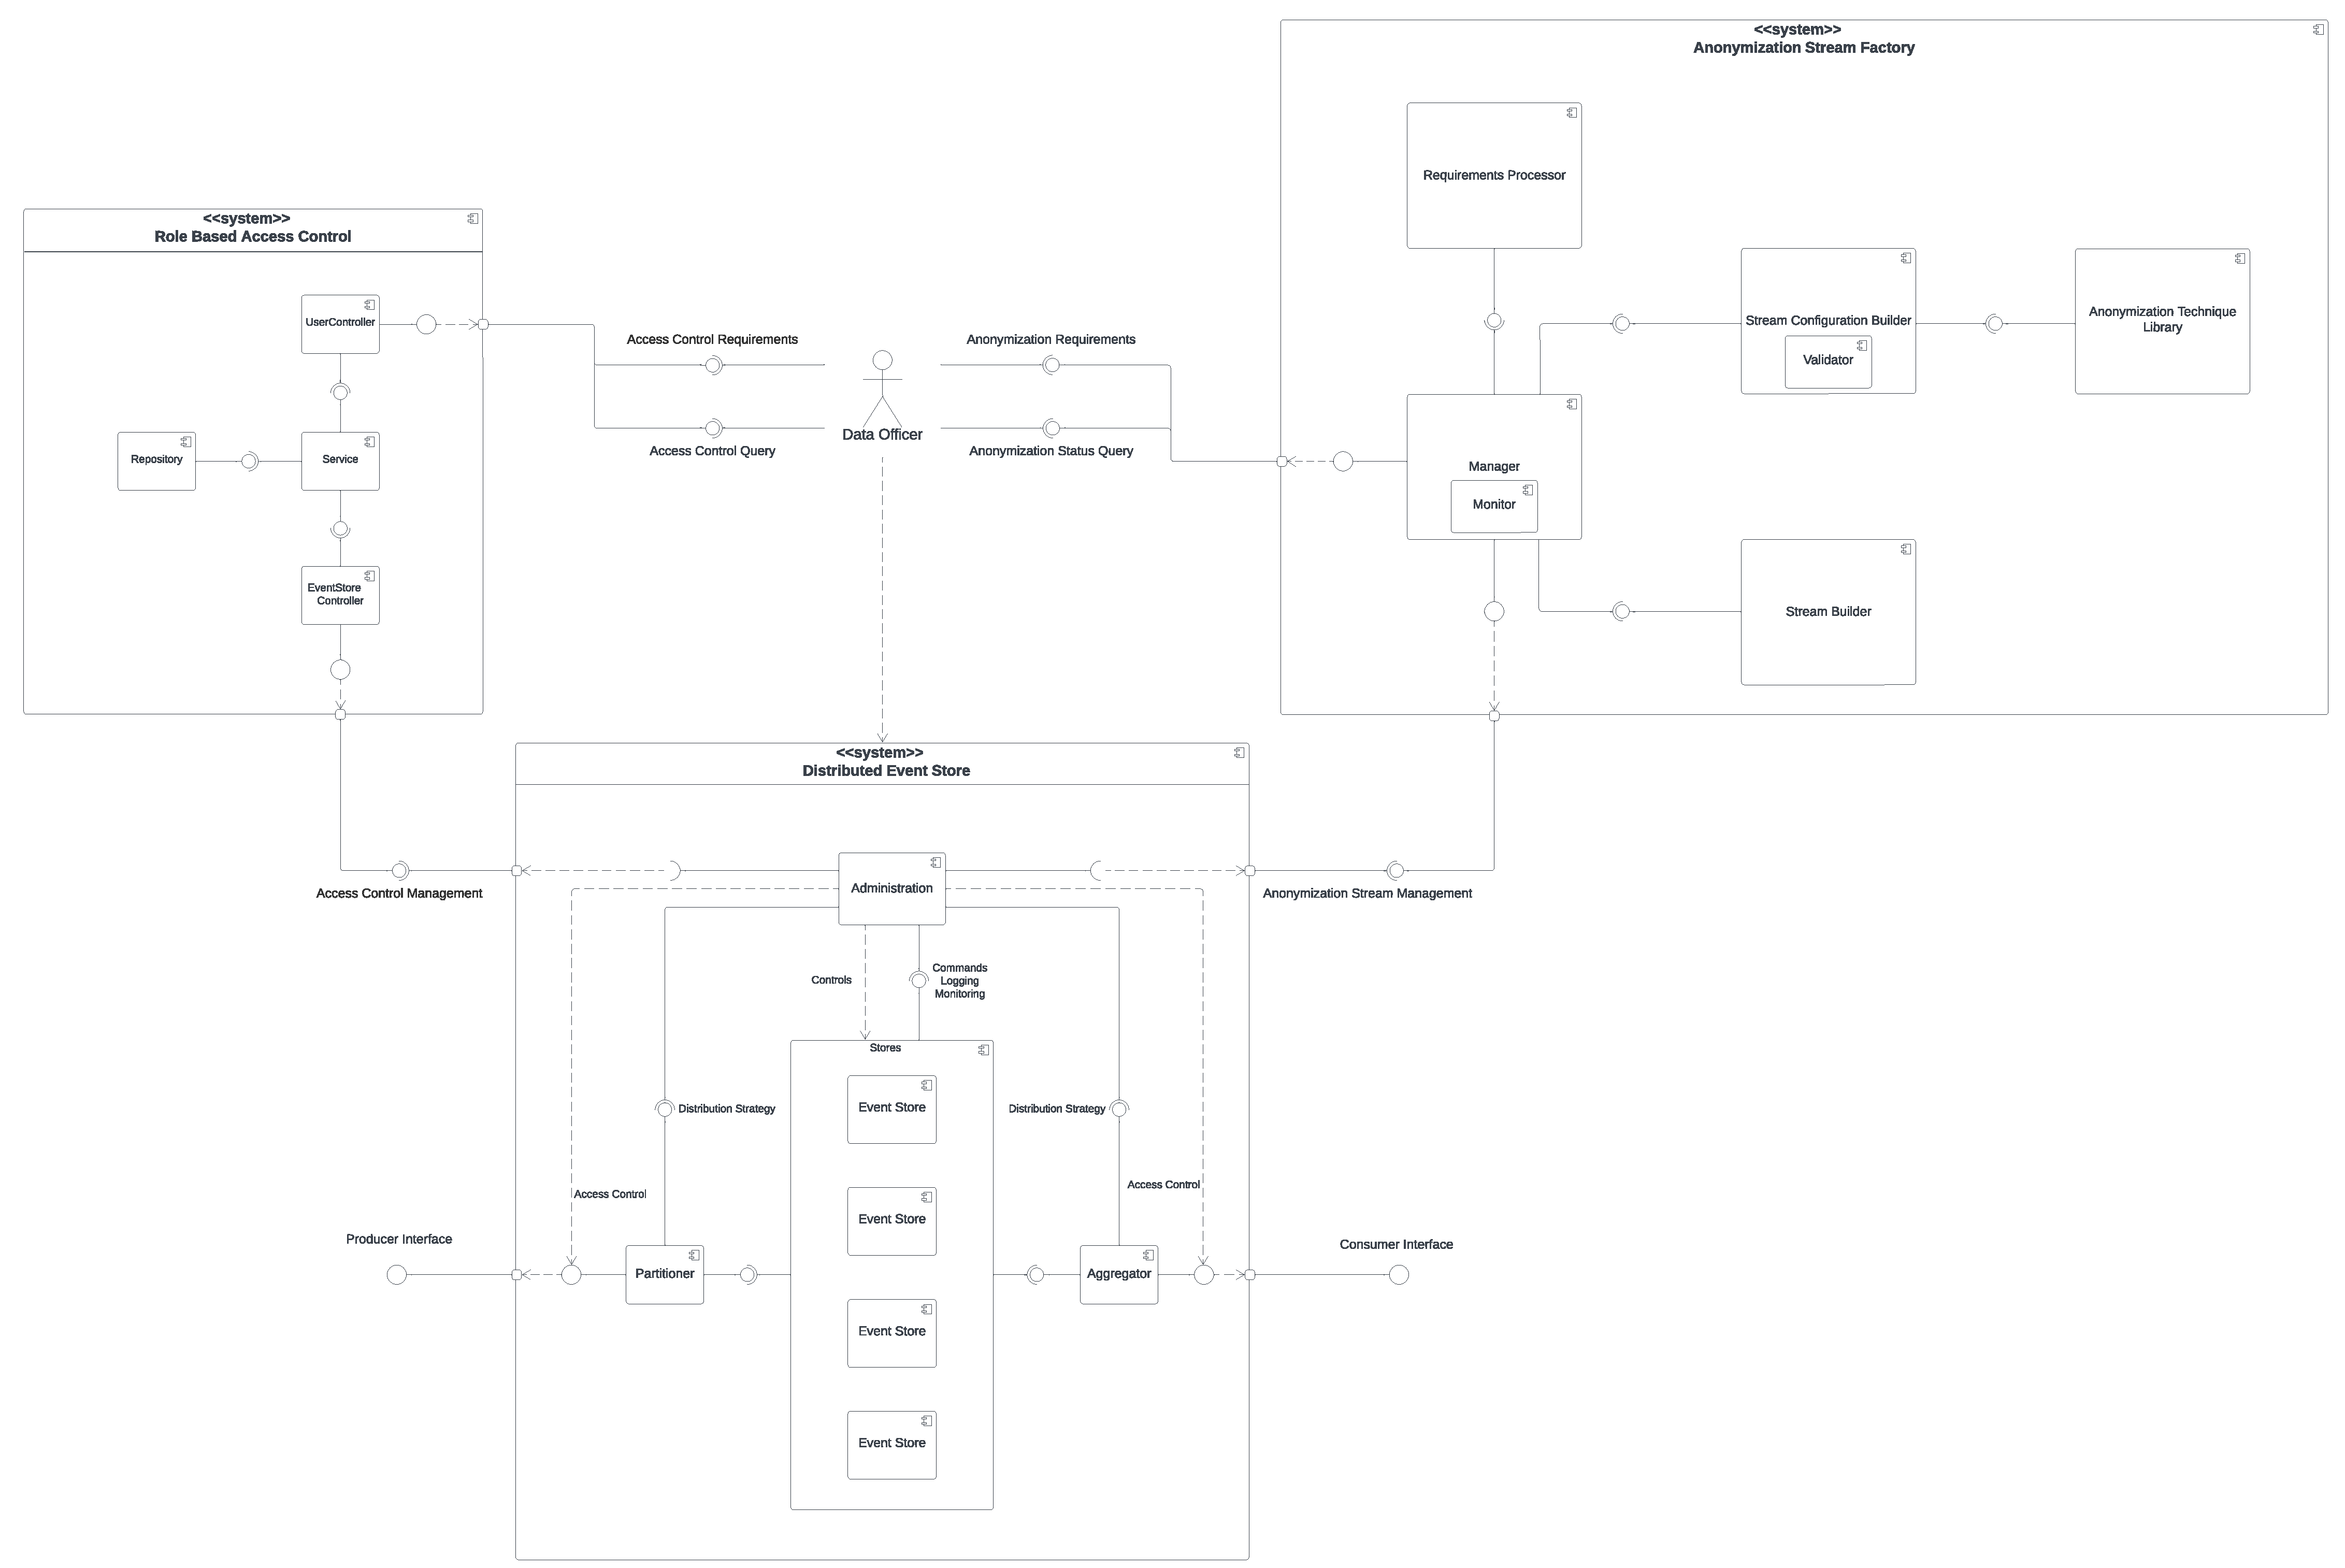
\includegraphics[width=\linewidth]{img/Complete_Component_Diagram.pdf}
    \caption{Full UML Component Diagram for the system as a whole.}
    \label{app:component_diagram}
\end{sidewaysfigure}


\addchap{Appendix B. Extended Version of the Experimental Results}


\end{document}
